%% 
%% Copyright 2007, 2008, 2009 Elsevier Ltd
%% 
%% This file is part of the 'Elsarticle Bundle'.
%% ---------------------------------------------
%% 
%% It may be distributed under the conditions of the LaTeX Project Public
%% License, either version 1.2 of this license or (at your option) any
%% later version.  The latest version of this license is in
%%    http://www.latex-project.org/lppl.txt
%% and version 1.2 or later is part of all distributions of LaTeX
%% version 1999/12/01 or later.
%% 
%% The list of all files belonging to the 'Elsarticle Bundle' is
%% given in the file `manifest.txt'.
%% 

%% Template article for Elsevier's document class `elsarticle'
%% with numbered style bibliographic references
%% SP 2008/03/01

%%\documentclass[preprint,10pt]{elsarticle}

%% Use the option review to obtain double line spacing
%% \documentclass[authoryear,preprint,review,12pt]{elsarticle}
%\documentclass[preprint,review,12pt]{elsarticle}
\documentclass[preprint,12pt]{elsarticle}

%% Use the options 1p,twocolumn; 3p; 3p,twocolumn; 5p; or 5p,twocolumn
%% for a journal layout:
%% \documentclass[final,1p,times]{elsarticle}
% %\documentclass[final,1p,times,twocolumn]{elsarticle}
% %\documentclass[final,3p,times]{elsarticle}
%% \documentclass[final,3p,times,twocolumn]{elsarticle}
%% \documentclass[final,5p,times]{elsarticle}
%% \documentclass[final,5p,times,twocolumn]{elsarticle}

%% For including figures, graphicx.sty has been loaded in
%% elsarticle.cls. If you prefer to use the old commands
%% please give \usepackage{epsfig}

%% The amssymb package provides various useful mathematical symbols
\usepackage{amssymb}
\usepackage{subfigure}
%% The amsthm package provides extended theorem environments
%% \usepackage{amsthm}

%% The lineno packages adds line numbers. Start line numbering with
%% \begin{linenumbers}, end it with \end{linenumbers}. Or switch it on
%% for the whole article with \linenumbers.
%% \usepackage{lineno}

%\journal{Physics Letters B}
\journal{NIM A}
\input def.tex
\input newcommands.tex

\begin{document}

\begin{frontmatter}
%---
\title{CALIS - a CALibration Insertion System for the \dsf\, dark matter search experiment}
%---
%\input uar-70d-frontpage.tex
\input frontpage.tex

%---
%\date{\today}
%---
\begin{abstract}
This report describes design, fabrication, commisioning and use of  a calibration source insertion system (CALIS) in \dsf\ experiment. CALIS  deploys radioactive sources into the liquid scintillator veto to characterize the detector response and detection efficiency of the \dsf\ Liquid Argon Time Projection Chamber used for dark matter detection, and the surrounding \lsvscintillatormass\ organic liquid scintillator neutron veto.
It was commissioned in September 2014 and used successfully in several campaigns to deploy gamma and neutron sources since then. A description of hardware and highlights from calibration analysis results are given below.

%In order to calibrate the detector response and detection efficiency of the \dsf\ Liquid Argon Time Projection Chamber used for dark matter detection and the surrounding \lsvscintillatormass\ organic liquid scintillator neutron veto, we designed, built and implemented a calibration source insertion system (CALIS), which allows to deploy radioactive sources into the liquid scintillator veto. 

%We report the first results of \dsf, a direct search for dark matter operating in the underground Laboratori Nazionali del Gran Sasso (LNGS) and searching for the rare nuclear recoils possibly induced by weakly interacting massive particles (WIMPs).  The dark matter detector is a Liquid Argon Time Projection Chamber with a \dsfactivemass\ active mass, operated inside a \lsvscintillatormass\ organic liquid scintillator neutron veto, which is in turn installed at the center of a \ctfwatermass\ water Cherenkov veto for the residual flux of cosmic rays.  We report here the null results of a dark matter search for a \dsfexpo\ exposure with an atmospheric argon fill.  This is the most sensitive dark matter search performed with an argon target, corresponding to a 90\% CL upper limit on the WIMP-nucleon spin-independent cross section of \dsflimit\ for a WIMP mass of \dsflimitmass.
\end{abstract}
%---
\begin{keyword}
%% keywords here, in the form: keyword \sep keyword

%% PACS codes here, in the form: \PACS code \sep code

%% MSC codes here, in the form: \MSC code \sep code
%% or \MSC[2008] code \sep code (2000 is the default)
Dark matter\sep WIMP\sep Noble liquid detectors\sep Low-background detectors\sep Liquid scintillators\sep radioactive source calibration

\PACS 95.35.+d\sep 29.40.Mc\sep 29.40Gx

\end{keyword}

\end{frontmatter}

\linenumbers
\setcounter{tocdepth}{2}
\tableofcontents

%% main text
%\section{}
%\label{}
%---
\section{Introduction}\label{sec:intro}\label{sec:introduction}

\mymarginpar{keywords and PACS are from our papers - need updates?}

\dsf\ is a Liquid Argon Time Projection Chamber (\lar\ \tpc), operated in Italy's Gran Sasso National Laboratory (LNGS) to search for nuclear recoils induced by weakly interacting massive particles (WIMPs). The first physics result was reported in \cite{Agnes:2015gu} based on 50 live data collection days with Atmospheric Argon (AAr), providing the most sensitive limit on a dark matter search using a \lar\ \tpc\ to date with a 90\% CL upper limit on the WIMP-nucleon spin-independent cross section of $6.1 x 10^{-44}$ cm$^2$ for a WIMP mass of 100 GeV/c$^2$.  %along with two other key results: ar bg can be suppressed for ton-scale experiments using \uar and efficiency of the veto 

A first WIMP search using argon extracted from underground sources (Underground Argon, UAr) has been reported in \cite{Agnes:2015_uar}, following the WIMP search with AAr. UAr has a lower concentration of the radioactive $\beta$-emitter $^{39}$Ar by a factor (1.4 $\pm$ 0.2) $\times\, 10^3$ relative to AAr. Calibration campaigns have been performed in the presence of AAr and UAr.

The \dsf\ apparatus is described in detail in \cite{Agnes:2015gu}. As shown in fig.~\ref{fig:wholeAssembly_insideDetectors}, it features a \lar\ \tpc\ surrounded by a 30 t liquid scintillator-based veto (LSV) system, placed inside a water Cerenkov veto detector (\wcv), both of which measure in-situ and suppress radiogenic and cosmogenic backgrounds. On the top of the \wcv\ is a radon-free clean room (CRH) housing the cryogenic supply system and electronics (Fig.~\ref{fig:CALIS_photos}). The \lsv's inside is accessible from CRH through four access ports, called organ pipes, which are closed by gate valves. 

%After this introduction the CALIS design requirements and hardware realization are described in Sec.~\ref{sec:hardware}. Calibration campaigns and some of their physics highlights are discussed in Sec.~\ref{sec:CalibCampaigns}, before concluding in Sec.~\ref{sec:Conclusion}.

\begin{figure}[htbp]
 \centering
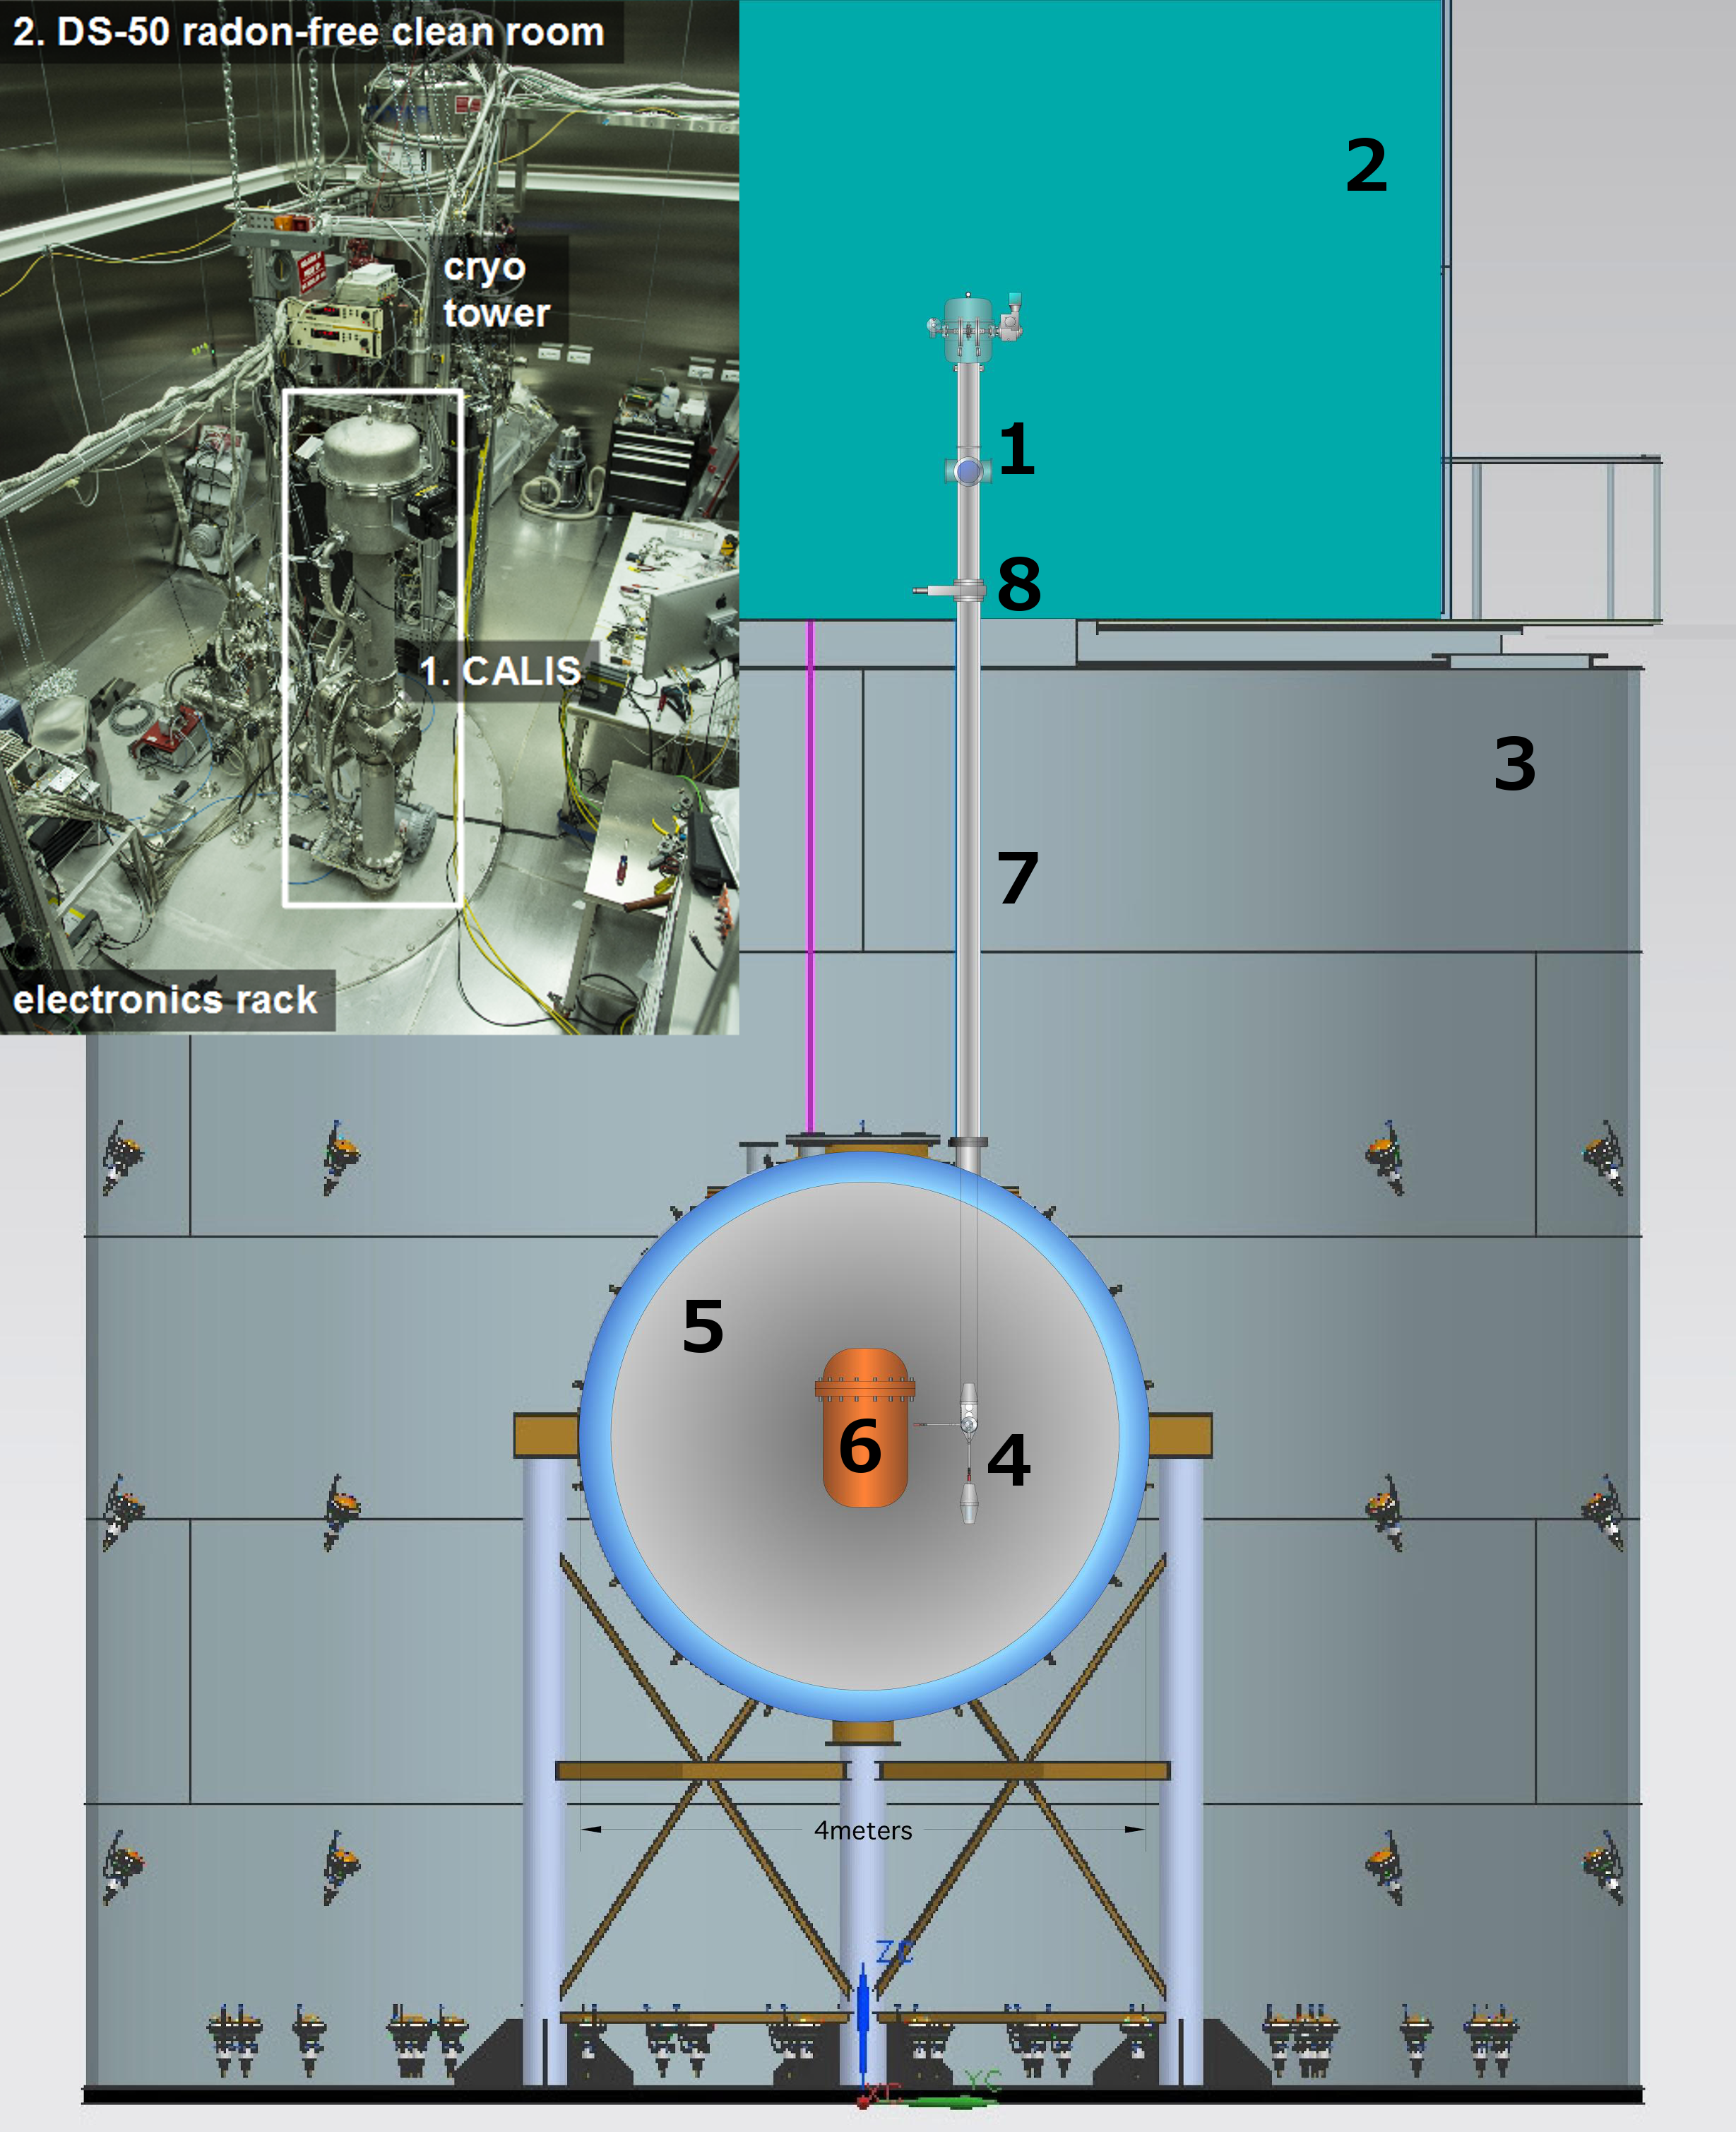
\includegraphics[width=0.95\textwidth]{Figures/DS50_with_CALIS}
\caption{A conceptual drawing of CALIS (1) installed in the radon-free clean room, CRH, (2) atop the water Cerenkov veto (\wcv, 3). The deployment device (4) which contains the source is deployed in the liquid scintillator veto (LSV, 5) next to the liquid argon time projection chamber's (\lar\ \tpc) cryostat (6). The clean room and the LSV are connected through four access ports, called organ pipes (only one of which is drawn in the above sketch (7)). All four organ pipes end in CRH at gate valves (8) which can be manually opened or closed. During normal operations all four organ pipes are closed. Not included in the sketch are tubes connecting the cryogenic systems in CRH to the cryostat in the \lsv\ \cite{Agnes:2015qyz}.\label{fig:wholeAssembly_insideDetectors}\label{fig:DS50_with_CALIS}}
\end{figure}

\begin{figure}[htbp]
 \centering
\subfigure{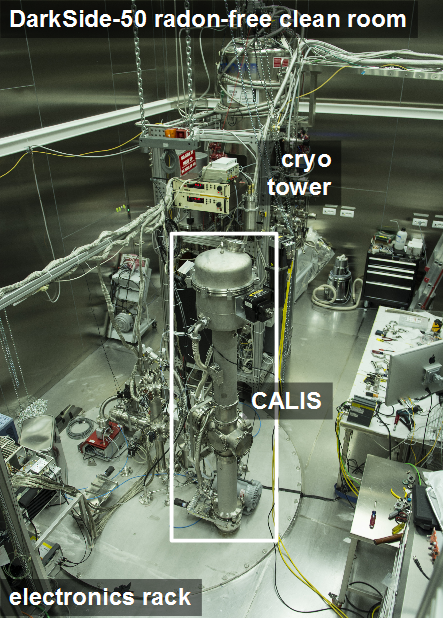
\includegraphics[width=0.335\textwidth]{./Figures/CALISinCRH_PetersComment.png}}
\subfigure{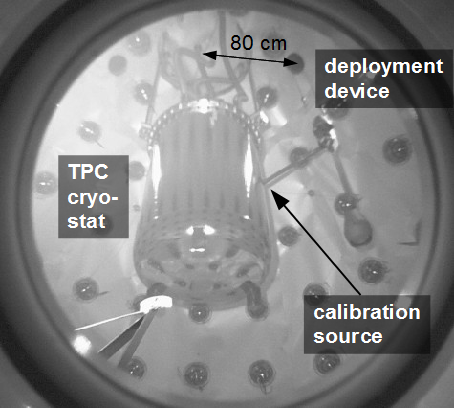
\includegraphics[width=0.52\textwidth]{./Figures/Next2Cryostat_80cm.png}}
\caption{\textit{Left}: CALIS after installation inside the radon-free clean room CRH. The organ pipe is 80 cm off-center with respect to the TPC's vertical Z-axis. \textit{Right}: Photograph taken with a camera looking upwards into the \lsv\ from the bottom. It shows the source deployment device deployed through one of the organ pipes visible on the top right. The arm is articulated and the source is next to the \lar\ \tpc's cryostat \cite{Agnes:2015qyz}.
\label{fig:CALIS_photos}}
\end{figure}


%time line plot, how did the veto change during the calibration campaigns - allowing for systematics studies.
%table on what was the goal of each campaign. What sources were used


%safety requirements

%design section
%installation: before, after


\section{Design Requirements \& Hardware Implementation} \label{sec:hardware}\label{sec:design_requirements}

\subsection{Purpose}
CALibration Insertion System (CALIS) deploys radioactive gamma and neutron sources inside the LSV to study and calibrate the detector response and neutron detection efficiency of the TPC and LSV. This complements and extends the physics reach of internal calibration sources and laser calibration. 
%The goal with the CALibration source Insertion System (CALIS) is to study and calibrate the detector response of the \tpc\ and the \lsv\ as well as the detection efficiency of internal neutrons interacting in the \tpc\ and \lsv\ using radioactive gamma and neutron sources. 

The center of the \lsv\ is about 6 m below the gate valve inside CRH
%=6145=70+120+400+3455+20+251+1372+457 from http://darkside-docdb.fnal.gov:8080/cgi-bin/RetrieveFile?docid=858&filename=NoFlyZone-DS50_vers02.pdf&version=14
 and the 15 cm diameter wide organ pipes are 80 cm off the \tpc\'s vertical z-axis as shown in Fig.~\ref{fig:CALIS_photos}. For \tpc\ calibration the radioactive source has to be positioned in immediate contact with the cryostat, in order to minimize rate losses through absorption in particular for low energy sources such as $^{57}$Co (122 keV). 

\subsection{Deployment \& Articulation Mechanism}\label{sec:DeploymentArticulation}
%focus on the mechanism --- protection provided by the housing is discussed below:
This requirement precludes a single cable solution deployed from within a glove box as has been used in several scintillator experiments \cite{Banks:2014hra, Huang:2013uxa}. %\cite{KamLAND-MiniCal, DayaBay_zaxis}. 
As shown in Figs. \ref{fig:CALIS_photos} and \ref{fig:CALISMechanism} the apparatus consists instead of the enclosure, which has been installed in CRH and the deployment device is attached to the housing through two stainless steel cables that are wound up on cable spools and allow the lowering of the device into the \lsv, next to the cryostat.
\begin{figure}[htbp]
 \centering
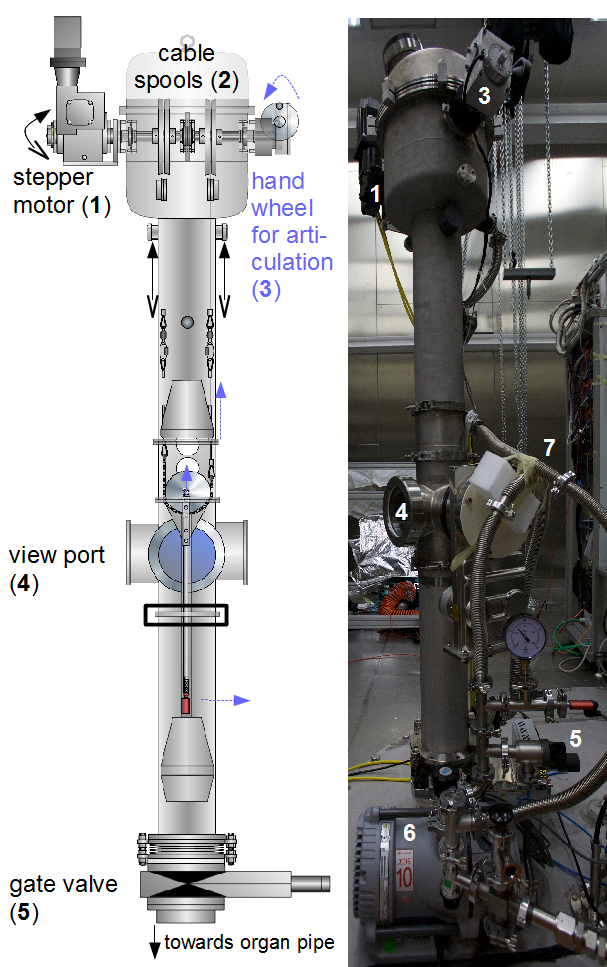
\includegraphics[width=0.8\textwidth]{Figures/CALIS_overview.png}
 %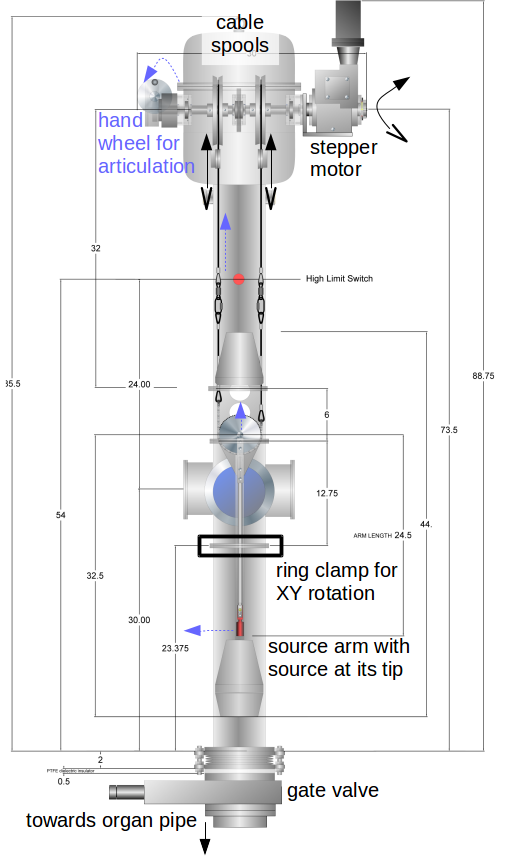
\includegraphics[width=0.68\textwidth]{Figures/CALISDimensions.png}
 %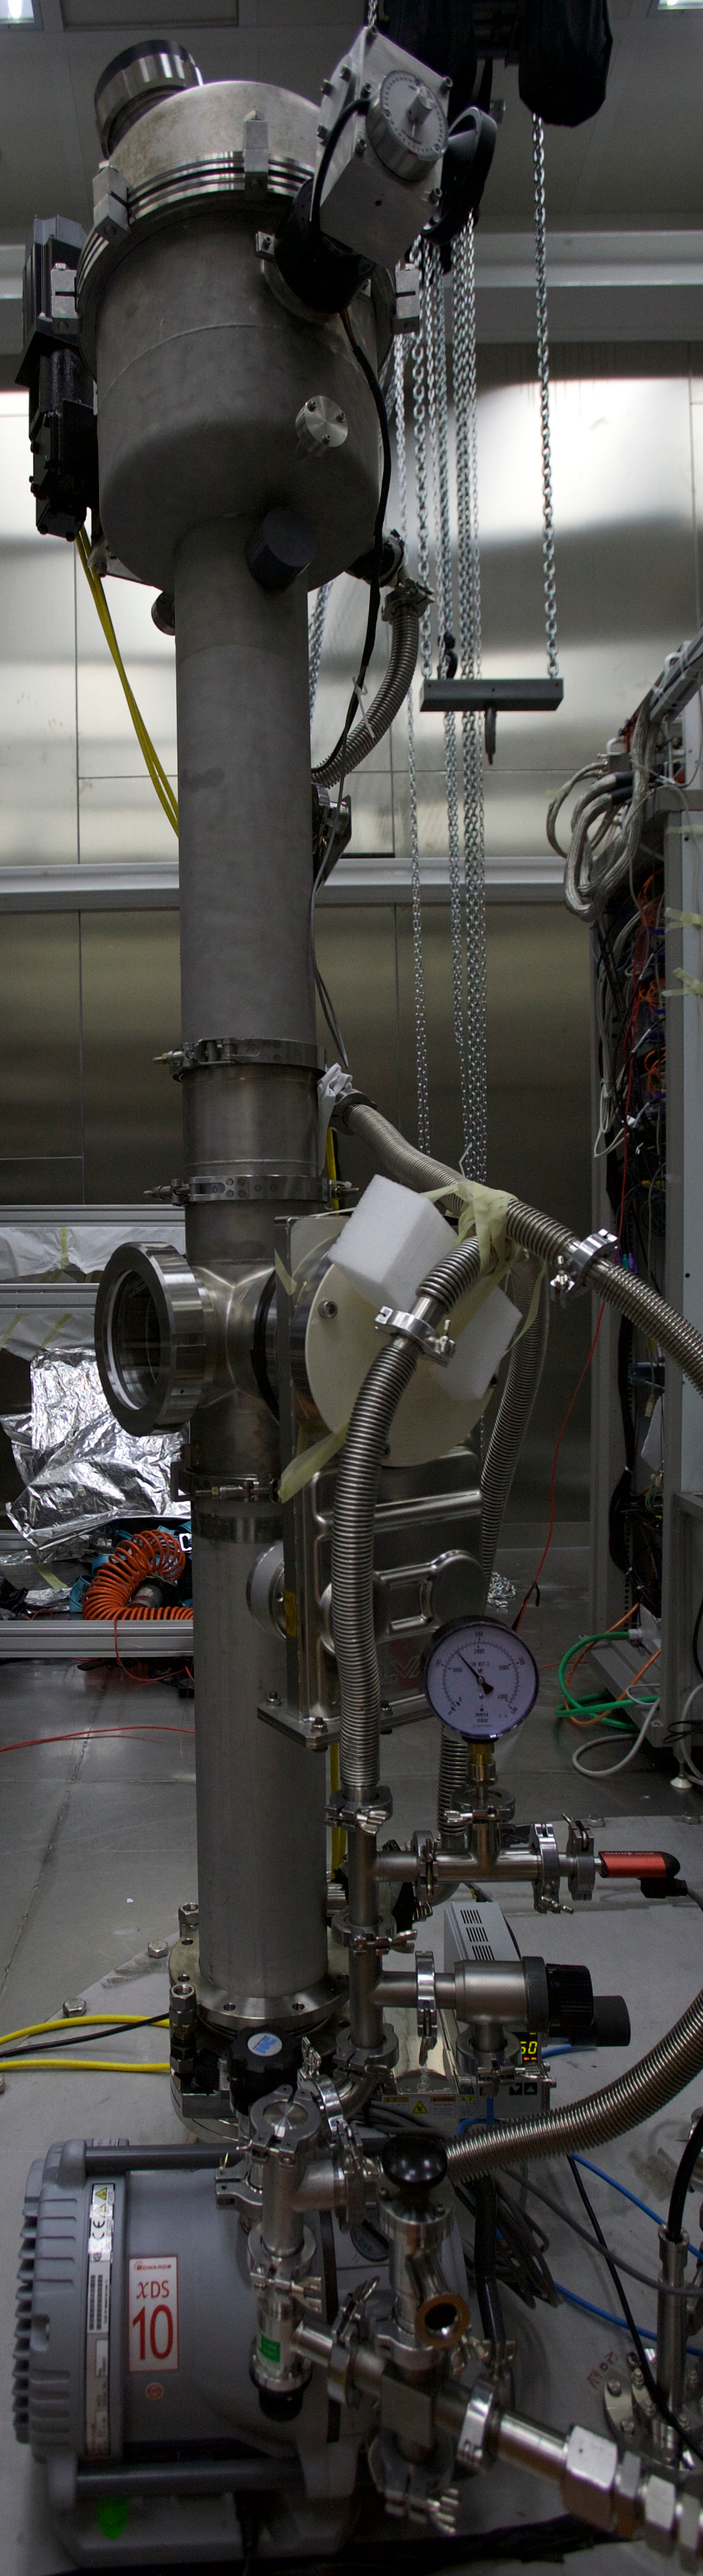
\includegraphics[width=0.30\textwidth]{Figures/CALIS_overview_IMG_3763.jpg}
 \caption{Mechanical drawing of CALIS showing the housing and the deployment device in its home position. The total height is approx.~240 cm including the gate valve.) The two modes of operation are illustrated: In order to move the deployment device down into the LSV or back up the stepper motor moves both cable spools (2) simultaneously. \textcolor{blue}{In order to articulate, the articulation wheel (3) is rotated manually, which affects only the right spool, thereby shortening the right cable with respect to the left cable thereby articulating the arm and lifting the pivot center.} The amount of lifting and the amount of rotations until a horizontal articulation is reached has been calibrated prior to installation in CRH (Sec.~\ref{sec:Testing}). In the photograph the vacuum pump (6) and tubing (7) are shown, which are part of the evacuation and purging system (Sec.~\ref{sec:EvacPurge}). \label{fig:CALISDimensions}\label{fig:CALISMechanism}\label{fig:gearDrawing}\label{fig:flushing_purging}
}
\end{figure}

\begin{figure}[htbp]
 \centering
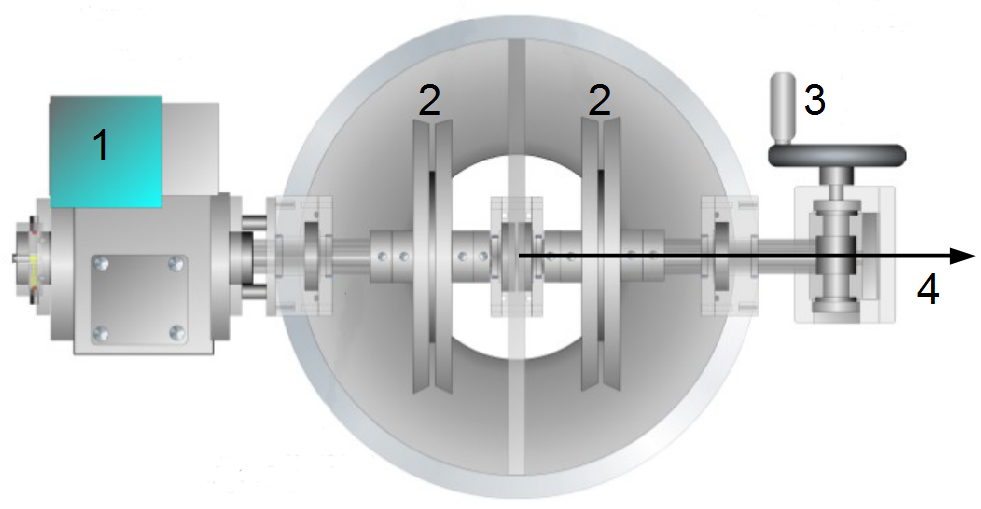
\includegraphics[width=0.9\textwidth]{Figures/gearDrawing_withNumbers}
  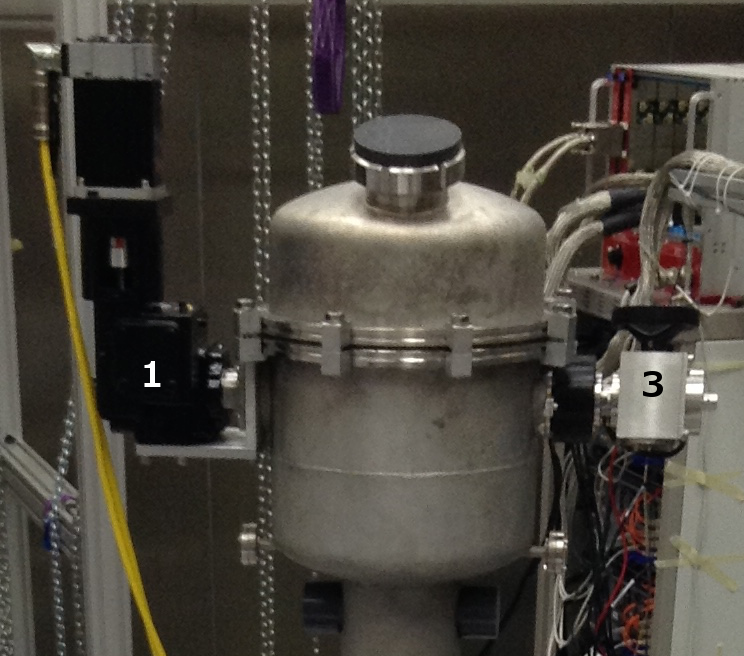
\includegraphics[width=0.46\textwidth]{Figures/CALIS_head.png}
  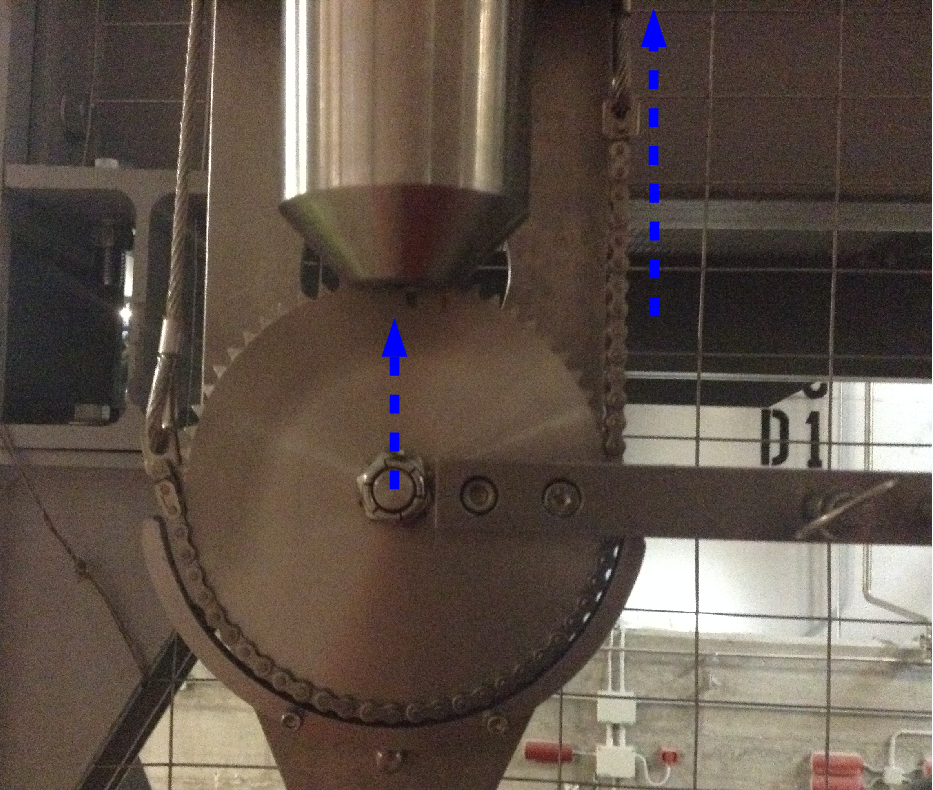
\includegraphics[width=0.48\textwidth]{Figures/gearArticulated.png}
  \caption{\textit{top}: Inside view of the drive mechanism's components seen from the top of CALIS. The stepper motor inside the motor housing (1) drives both cable spools (2) concurrently, thereby lowering the calibration device into the \lsv. An absolute encoder provides the current position of the deployment device. The hand wheel (3) turns the right spool only, thereby transfering the rotation of the articulation wheel into a (de)articulation of the source arm (\textit{bottom right}). The arrow (4) in the sketch points in the same direction as the horizontally articulated arm. The chain has a guard rail, that ensures that the chain can never come off the gear.}
  \label{fig:sourceArmRotation}
\end{figure} 

The stepper motor moves both cable spools concurrently and sends the deployment device into the \lsv. An absolute encoder provides its current position, even in the absence of power. The stepper motor is controlled via a simple graphical LabVIEW interface, run on a dedicated laptop, in which the current z-position is shown and a target z-position can be provided by the operator. Z-positions are given in motor step counts, an arbitrary unit which has been calibrated outside CRH in meters (Fig.~\ref{fig:z_test}) and relative to the TPC using the t-drift distribution of calibration data (Fig.~\ref{fig:SourcePosition}).

\begin{figure}[htbp]
 \centering
 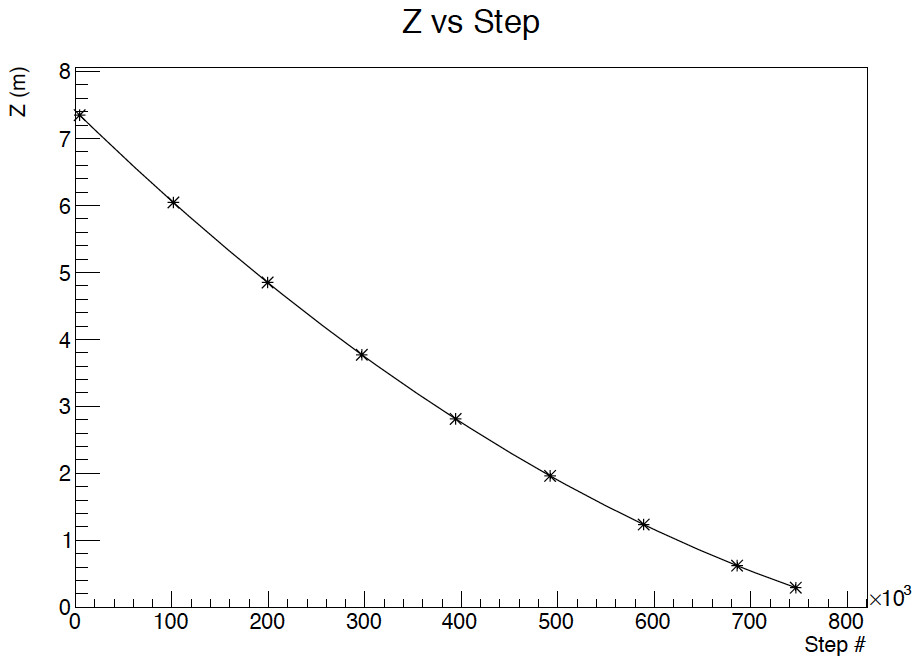
\includegraphics[width=0.65\textwidth]{Figures/Z_positioning_test}
 \caption{Plot of the z position of the deployment device versus the step position of the motor. The non-linear correspondence between the number of steps and the length of cable deployed arises as follows: As the cable winds around the spool, the winding radius changes, increasing as the deployment device is lifted and decreasing as it is lowered. A motor step count corresponds to a fixed angular distance \textit{d$\theta$}, yet the amount of cable deployed during this motor step count is \textit{winding radius $\cdot$ d$\theta$}. As the winding radius changes as a function of z position, the fraction of deployed cable per motor step count changes.}
 \label{fig:z_test}
\end{figure}

\label{sec:Nonlinearity:MotorStepCounts}
Articulation of the arm is done manually via the articulation wheel. This affects only the cable spool close to the articulation wheel, the left one in Fig.~\ref{fig:sourceArmRotation}, thereby shortening the left cable with respect to the right cable and engaging the gear through a chain (Fig.~\ref{fig:sourceArmRotation}). As a result the arm is articulated and the pivot center is lifted. The non-linearity arising from the change in winding radius on the cable spools affects also the amount of rotation required by the hand wheel for horizontal articulation of the source arm.
The degrees on the articulation wheel corresponding to a horizontal articulation have been calibrated as a function of cable length deployed prior to installation in CRH.

Articulation and a movement in z-direction are mutually exclusive since the articulation of the arm leads to more wound up cable on the spool close to the articulation wheel with respect to the other. If then in deployment mode both spools would be rotated simultaneously with the same angular speed, the cable close to the articulation wheel would wind up faster than the other, which would lead to a build up of difference in cable length and the deployment device would only be hanging on one cable. In order to avoid an imbalanced z-movement the arm has to be dearticulated fully before a change in z-position can be initiated. This is enforced by an electric switch preventing z-movement, which is disengaged only when the arm is fully dearticulated (vertical). 

%Discussion:
% why no permanent tube?
% To complement studies of nuclear recoils with neutron sources ($^{241}$Am$^{9}$Be and $^{241}$Am$^{13}$C), it is planned to deploy a 

\subsection{CALIS enclosure \& Scintillator}

Besides providing mechanical support for the deployment device via the cable spools, the CALIS enclosure is an important interface between the radon-free clean room CRH and the \lsv, through which sources are exchanged. 
The enclosure protects the liquid scintillator (LS) and eliminates human contact with any traces of harmful  liquid scintillator vapor (Fig.~\ref{fig:CALISMechanism}). It plays the same role as a glove box for similar calibration systems yet with a narrower foot print inside CRH. The liquid scintillator is a mixture of PC and TMB\footnote{The concentration of TMB has varied during campaigns (see Sec.~\ref{sec:CalibCampaigns}).} with the wavelength shifter PPO \cite{Agnes:2015qyz}. %\cite{vetoPaper}. 
It may not get exposed to oxygen or water as is present in normal clean room air. Contamination of LS with $^{222}$Rn and its long-lived radioactive daughters has to be avoided, too. 

Going up from the gate valve on which CALIS has been installed, there is a teflon disk that can electrically isolate CALIS from ground, even though during normal operations the CALIS housing is connected to ground. A tripod with a bellow has been used to vertically align the enclosure right after installation on the gate valve. The bellow is connected to a 59.4 cm long cylindrical stainless steel enclosure pipe. It has the same diameter as the organ pipe (15 cm) and connects to the view port above by a ring clamp, which plays a critical role in XY rotations (see Sec.~\ref{sec:XYrotation}). The view port can be opened for handling the source arm and exchanging sources. Everything above the ring clamp forms the upper assembly. It features a stainless steel cylindrical enclosure that houses the cable drive mechanism, including the cable spools, the stepper motor and the articulation mechanism already described in Sec.~\ref{sec:DeploymentArticulation}. 

\subsubsection*{Vacuum evacuation (flushing) and nitrogen purging system}\label{sec:EvacPurge}
One of the most important safety features of this system is making sure that the TMB and PC residue on the device are extracted from CALIS prior to opening access ports to exchange source or arms. This is  important for safe working conditions inside CRH as well as for the scintillator and radiopurity. 

After the insertion of the source arm and closure of the view port the inside of the CALIS housing is filled with normal air, that is damaging to the scintillator. A sequence of evacuations and nitrogen purges reduces the fraction of air including its contaminants (water vapor, oxygen, radioactivity) to negligible levels. Only after this sequence is finalized the gate valve is opened and the deployment device is introduced into the LSV. Evacuation is achieved with a vacuum pump and exhaust air is removed through dedicated vent lines (Fig.~\ref{fig:flushing_purging}).

At the end of a calibration campaign, after the deployment device has returned to its home position inside the housing and the gate valve has been closed, scintillator vapor and in particular TMB have to be removed prior to opening the view port. Again a sequence of evacuations and nitrogen purges is employed. By lowering the pressure inside of CALIS below the vapor pressure of TMB and PC, the scintillator evaporates and gets removed through the vent line of the vacuum pump. Once the pressure inside the housing stays consistently below the vapor pressure of TMB all scintillator has been removed and the view port can be opened to access the source arm.
 
%\begin{figure}[htbp]
%\centering
% 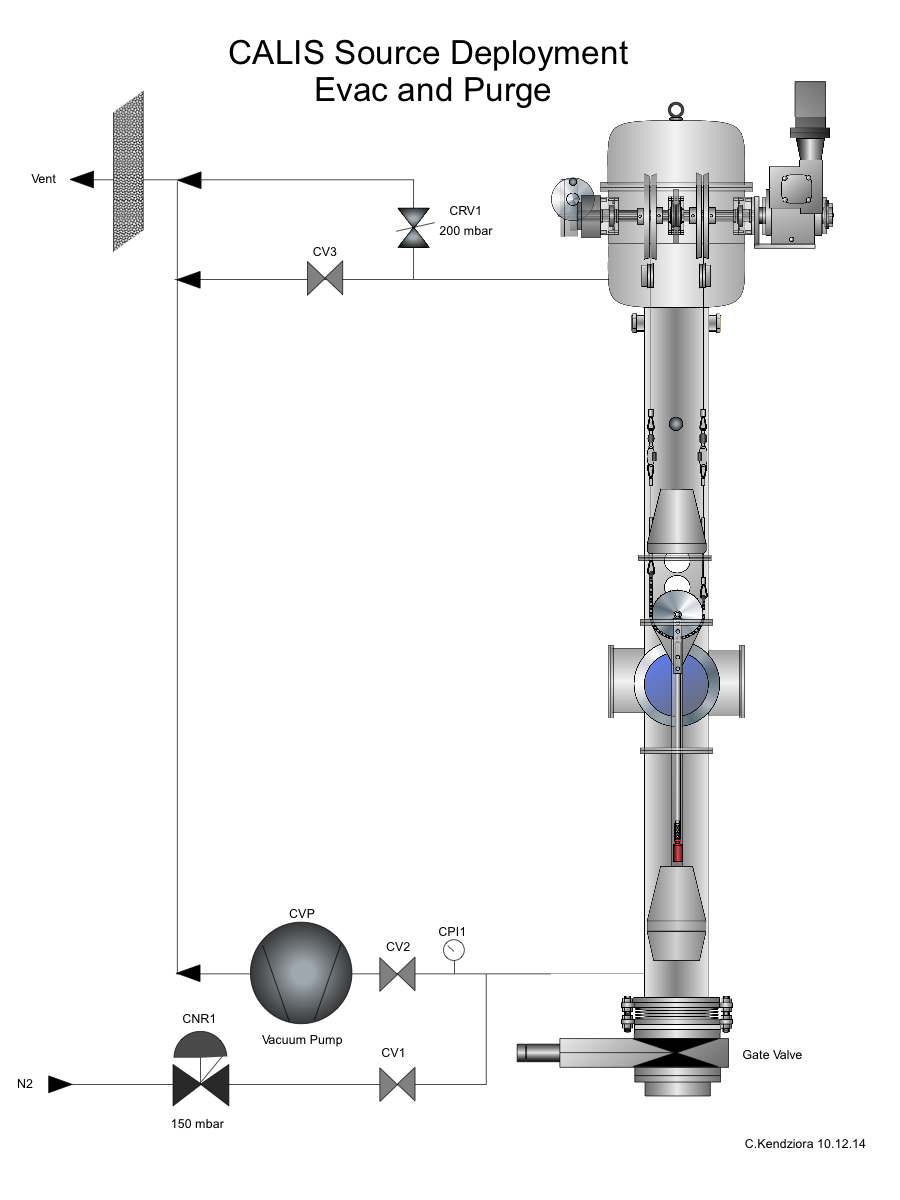
\includegraphics[width=0.73\textwidth]{Figures/GasSystem.png}
% 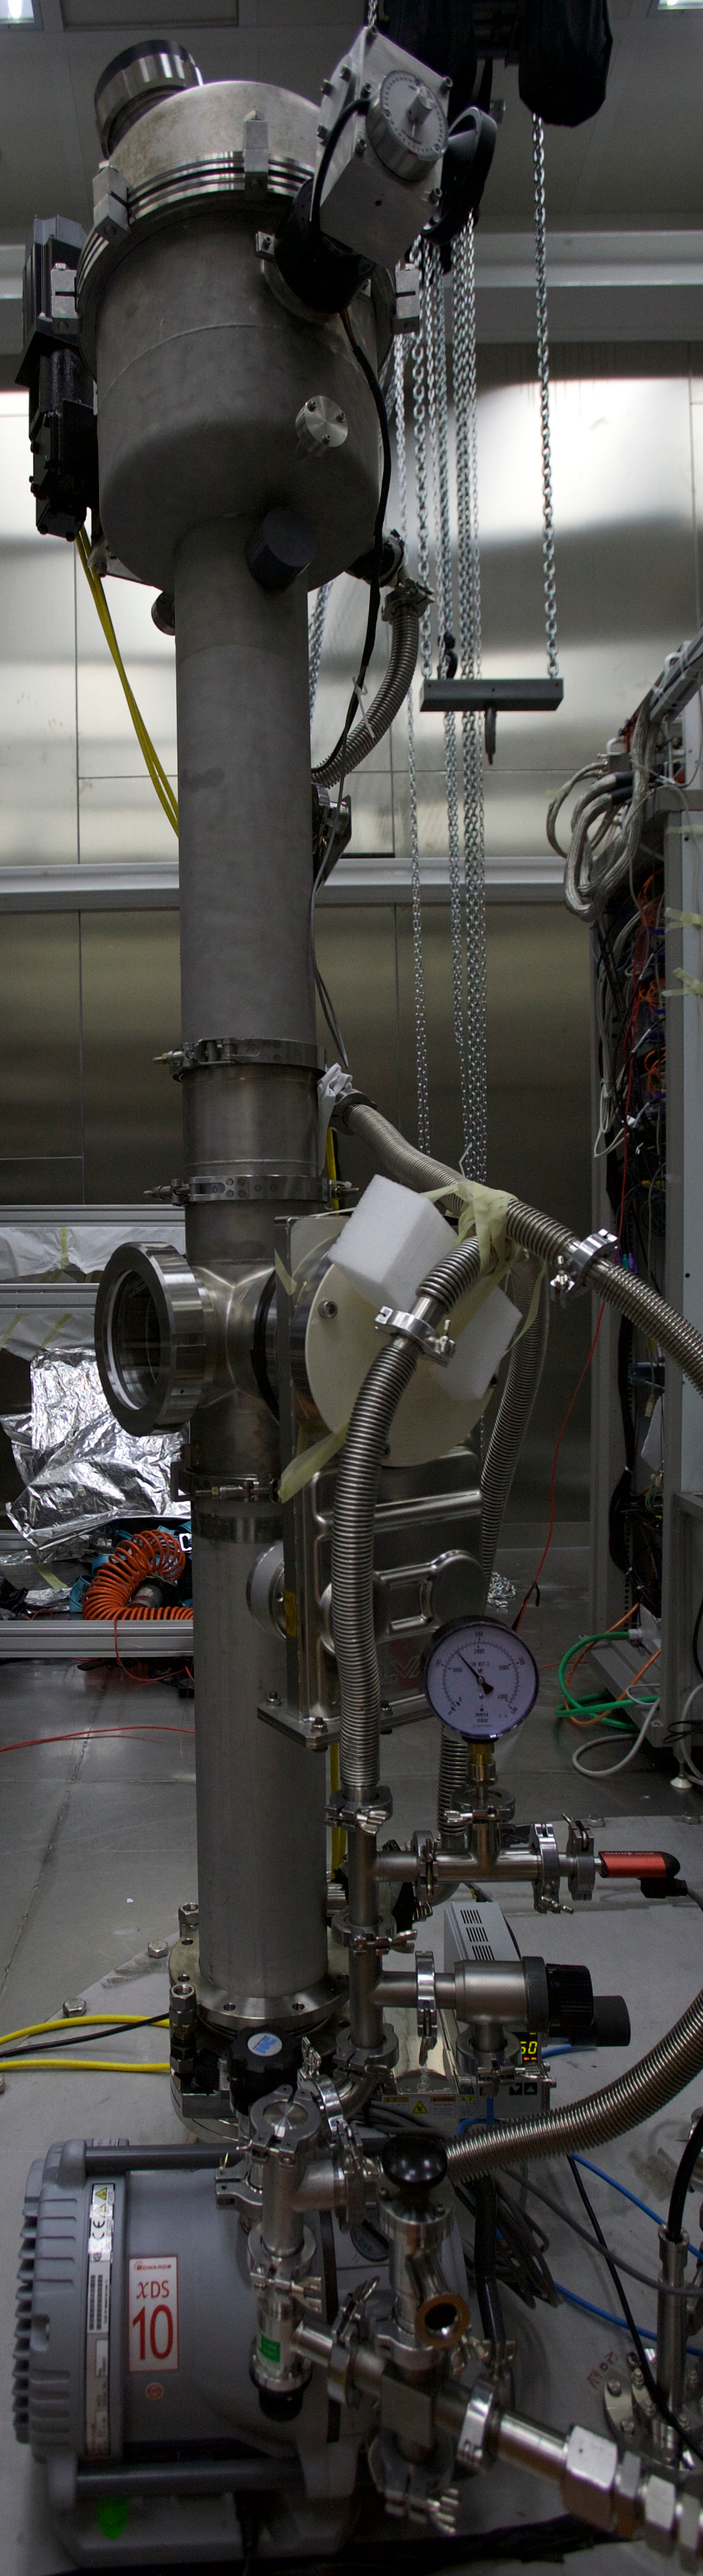
\includegraphics[width=0.25\textwidth]{Figures/CALIS_overview_IMG_3763.JPG}
% \caption{Flushing and nitrogen purging system.}
% \label{fig:flushing_purging}
%\end{figure}

\subsubsection*{Material compatibility}
All materials that come in contact with the scintillator veto are made of stainless steel and teflon except for the sealing o-rings which are made of viton.  All three materials are certified materials for contact with scintillator components TMB and PC.

\subsection{Deployment device}
The deployment device (Fig. \ref{fig:CALISMechanism}) contains the support structure for the arm which holds the source at its end. The device is equipped with tapered cones on the top and bottom that ensure that the ends do not get snagged on inner edges of the organ pipe as it is moving up and down. It is attached to the housing by two cables.  Swivel hooks are employed in the attachment of the cables to the deployment device that allow the cables to move freely and not get tangled. 
There are two weights built into the device, one cylindrical in the conical cap above the rotation gear mechanism and one inside the cones at the bottom end of the device. Both help to minimize any lateral motion or oscillations during deployment and articulation and dearticulation especially. It also ensures smooth motion of the deployment device into the organ pipe and back to the home position inside the housing.

\subsection{Source holder and arms}
A source arm and the source holder are attached to the articulation gear (Fig.~\ref{fig:SourceHolder}). Different arm lengths have been prepared with a maximum arm length of 62 cm, the arm length thereby being measured from the pivot point of the rotation gear to the tip of the source holder. This arm length allows the source to be placed in immediate contact with the cryostat (Fig.~\ref{fig:CALIS_photos}, right), as the center axis of the organ pipe is 80 cm from the TPC center and the cryostat has an outer radius of 32 cm. The 62 cm arm was used for deployments in the past calibration campaigns (Sec.~\ref{sec:CalibCampaigns}). Inside the source holder the radioactive source is placed, pressed to the tip and held in place via a spring during deployment, articulation and dearticulation. The source holder is sealed such that no liquid scintillator can enter during the deployment. This has also been verified during each source extraction and no traces of liquid have been found on its inside.

\begin{figure}[htbp]
 \centering
  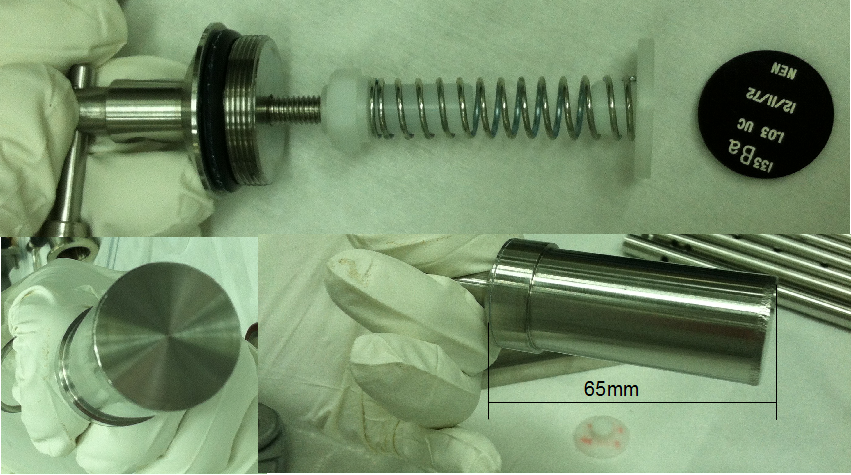
\includegraphics[width=0.7\textwidth]{Figures/SourceHolder.png}
  \caption{Source holder that connects to an arm and to the articulation gear of the deployment device. The source, here a $^{133}$Ba source, is pressed to the tip of the source holder via a spring.}
  \label{fig:SourceHolder}
\end{figure}
\subsection{Hardware details and safety features}
CALIS offers various safety features to ensure that the device runs smoothly, no components are lost inside the detector, avoid any contamination of the detector by dirty or incompatible materials, maintain pressure and avoid introduction of oxygen or water in contact with the LS and TMB. %, operation in the volume that excludes possibility of contact with PMTs or light pulsers (pacman) attached to each PMT.

\begin{description}

\item[Drive mechanism:]
In the event of a power failure, the magnetic break ensures there is no movement of the pig. The torque of the servo motor is limited in case of an unexpected load. 

The speed reducer (gears) is a double worm gear design. The primary worm gear has a 50:1 reduction and the secondary worm has a 82:1 reduction. The input speed of the servo motor is 2400 RPMs and the output is 0.6 RPM and has the weight capacity of 148 lbs. In the event of a power failure the speed reducer has the ability to hold the load at any position without back drive. The speed of the motor has been limited to 0.4\,cm/s which minimizes any lateral oscillation of the pig during lowering and raising the source. Additionally, this is the maximum speed at which the motor is not overheating.


\item[Cable strength:]
The cables holding the pig have been rated for loads over 590\,kg, while the weight of the deployment device is at the level of 10-15\,kg so well below the breaking strength of the cable. 

\item[Cable length:]
The cable length has been established so that the maximum depth at which the pig can be deployed is above the level of the PMTs inside the LSV. In case, the command is given to deploy to greater depth, the cable completely unwinds and then rewinds in the opposite direction, which then effectively retracts the pig to a higher z-position until the preset motor count of steps is reached. 

\item[Manual retraction system:]
In the unlikely case of a complete motor failure while the source is deployed, it is possible to manually retract the pig back to its home position and close the gate valve. The motor is disengaged, and wrench is used to manually wind the cable back onthe spools and retract the pig back above the gate valve. 
   
\item[High limit switch:]
A high limit switch is a hardware interlock, that prevents the deployment device to hit the cable spools and gears, should it pass beyond the home position in the CALIS housing (Fig.~\ref{fig:CALISMechanism}). 

\textit{Neither the manual retraction system had to be used so far nor has the high limit switch been activated during calibration campaigns.}
    
\item[Light and leak tightness of CALIS:]
When the deployment device is next to the cryostat the gate valve is open and we take also data with the LSV. A prerequisite is that the housing is absolute light tight and pressure leak tight. All view ports have light tight covers for when the organ pipe gate valve is open. Both light and leak tightness has been extensively validated throughout the manufacturing process until including commissioning (Sec.~\ref{sec:Commissioning}).

\item[Securing of the source]
All connection points for the source and arm have been secured with two push locking pins that cannot be disengaged without a person pressing the pin (Fig.~\ref{fig:sourceHolder_locking}). In addition, the source holder and the two locking pins will all be tethered from outside the view port until they are locked in place eliminating the possibility of accidental falling into the inside of the CALIS housing.

\end{description}
	
%%%%%%%%%%%%%%%%%%%%%%%%%%%%%%%%%%%%%%%%%
%%%%%%%%%%%%%%%%%%%%%%%%%%%%%%%%%%%%%%%%%

\begin{figure}[htbp]
 \centering
 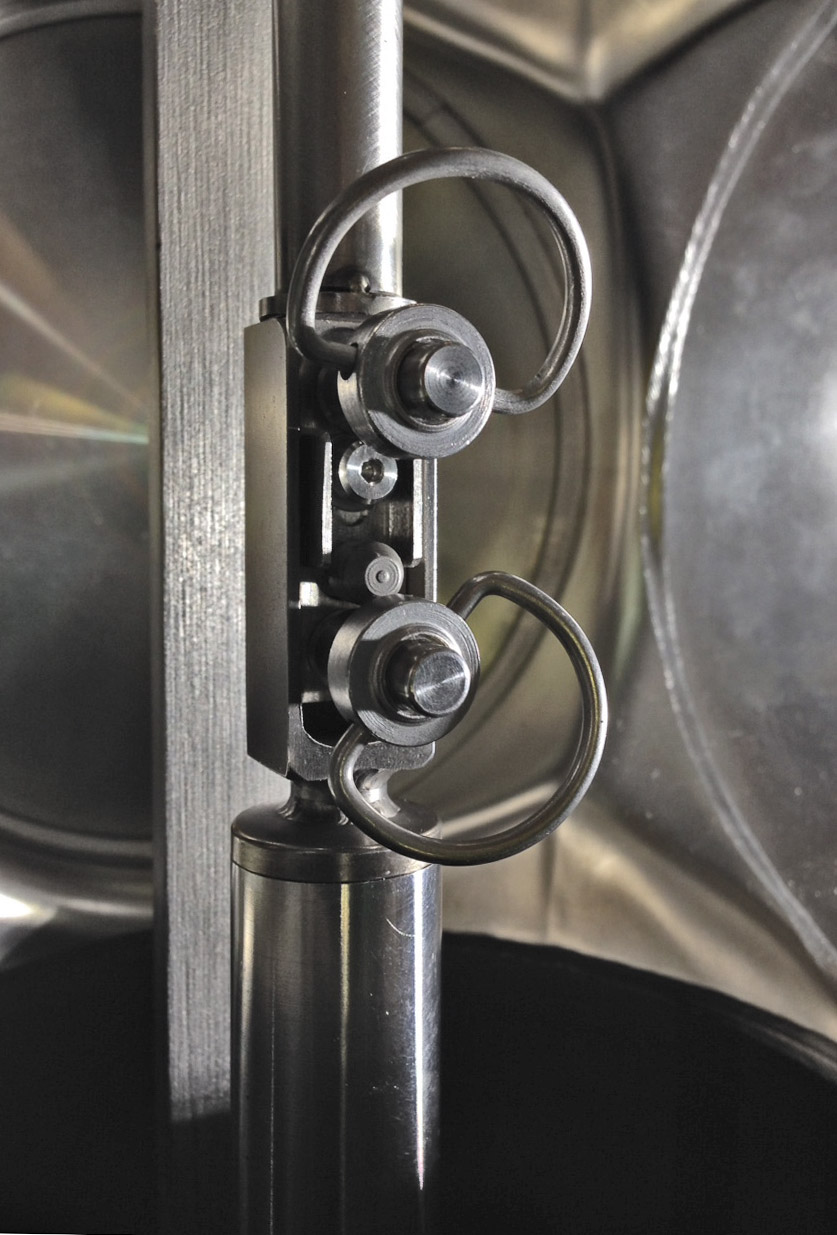
\includegraphics[width=0.3\textwidth]{Figures/sourceHolder_locking}
 \caption{Locking mechanism for the source holder. This photo shows two push pins that ensure that the sliding pin stays in place and the source holder cannot under any circumstances get detached from the arm.  The only way to remove the push pins is to depress buttons on each of them by hand.}
 \label{fig:sourceHolder_locking}
\end{figure}

%\begin{figure}[htbp]
% \centering
 % \includegraphics[width=7in]{Figures/sourceAttachmentParts}
%  \caption{Components of the source attachment mechanism. Central image shows how the pin that holds the source holder slides down and prevents the %source from getting loose.  The slide pin is locked in place by two push pins shown in Fig. \ref{fig:sourceHolder_locking}}
%  \label{fig:sourceAttachmentParts}
%\end{figure}

\subsection{Degrees of freedom of the system}

CALIS has the capability to deploy sources at various positions inside the LSV. Besides the movement along z up to the maximum cable length, there is the possibility to articulate at an angle of $\theta$ between 90$^{\circ}$ and 180$^{\circ}$, where $\theta$ is the zenith-angle (Fig.~\ref{fig:coordinate_system}). Degrees between 0$^{\circ}$ and 90$^{\circ}$ are excluded because the end of the articulation chain is reached at an angle of 90$^{\circ}$ (see Fig.~\ref{fig:sourceArmRotation}).

\begin{figure}[htbp]
 \centering
  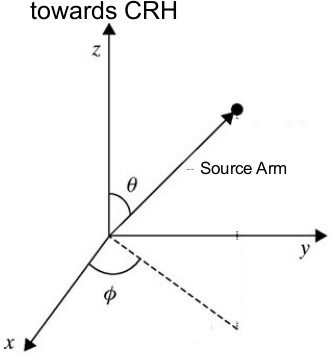
\includegraphics[width=0.4\textwidth]{Figures/coordinate_system}
  \caption{Spherical coordinate system used for establishing the direction of the rotation of CALIS-III and the articulation of the source arm. $\theta$ is kept at 90$^{\circ}$ when arm is articulated, and at 180$^{\circ}$ when dearticulated. $x$-axis is the direction toward the center of the detector. }
  \label{fig:coordinate_system}
\end{figure} 

\subsubsection{Rotation in the XY plane}
Below the view port is a sealed connection that has an o-ring seal and uses a ring clamp to compress the seal. The clamp can be slightly loosened to allow the assembly above and including the view port to be rotated with respect to the lower assembly and the detector. This rotation in the XY plane can even be performed while the gate valve is opened and the deployment device is deployed next to the cryostat, since the seal is helium leak and light tight even when loosened.

In principle a rotation in 360$\circ$ can be done, except when the arm would interfere with the cryostat. This has been used in one of the calibration campaigns to deploy a neutron source directly next to the cryostat and rotated away by 90$\circ$ in order to study optical shadowing effects from the cryostat (Sec.~\ref{sec:CalibCampaigns}). 

\mymarginpar{My impression is that a drawing to scale with the cryostat, the TPCthe organ pipe and the source arm would be good here}

For articulation, there is currently a choice of three arm lengths---40.31\,cm,  57.15\,cm and 62\,cm.  

Each of these lengths are measured from the center line of the organ pipe to the end of the source holder.  The arm lengths, 57.15\,cm and 62\,cm are intentionally made too long as they will be used to determine the exact location of the cryostat; some uncertainty in the cryostat's z and lateral position exist at the level of 3 - 4\,cm. The organ pipe we intend to use is 81\,cm distant from the cryostat center (and the geometric center of the LSV sphere) as measured from the center line of the organ pipe. The cryostat is 32\,cm in radius, which leaves a distance of $\sim$49\,cm to be reached  by the arm.


\begin{figure}[htbp]
 \centering
  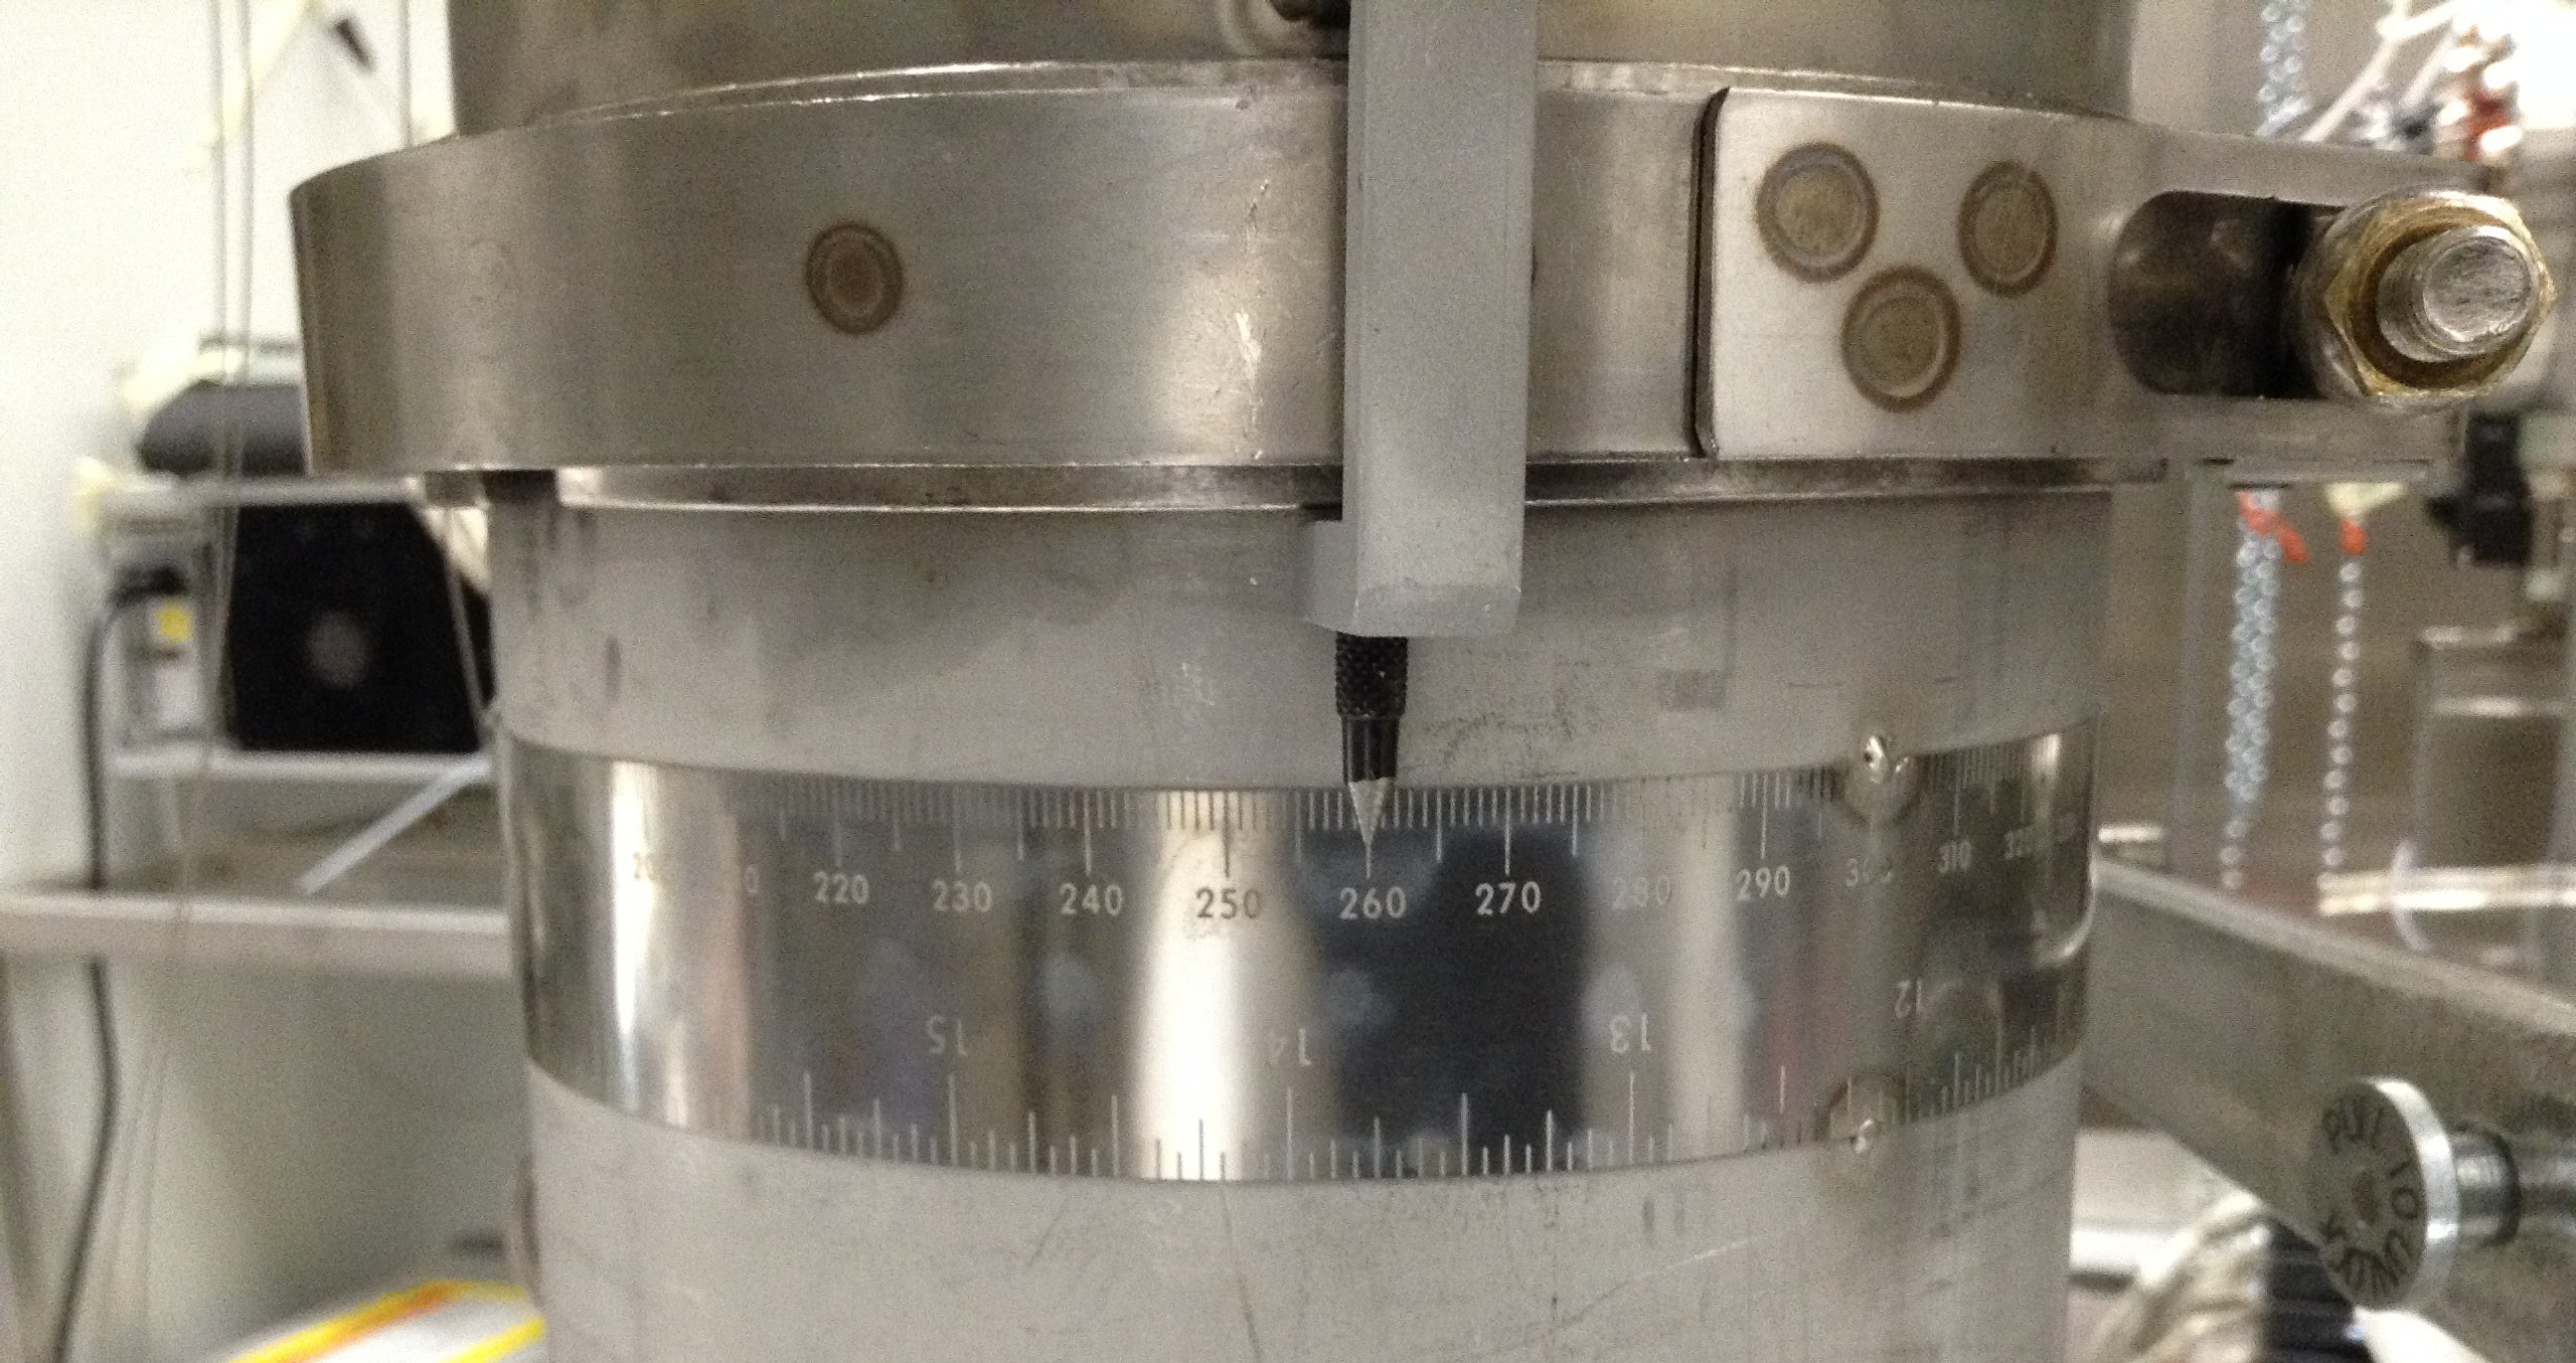
\includegraphics[width=0.7\textwidth]{Figures/RingClamp_WithPin_IMG_2669.JPG}
%  \includegraphics[scale=0.5]{Figures/RingClamp.jpg}
  \caption{Ring clamp  with the angle measuring strip shown below. In order to perform azimuthal rotation, the ring clamp is slightly loosened, and the entire upper assembly is rotated with respect to the lower assembly, along with the deployment device. The angle of rotation is read out from the strip that goes around the pipe. The strip is in mm, which has then been calibrated in degrees.}
  \label{fig:ring_clamp}
\end{figure} 

\subsubsection{``No fly'' zone}
Right above the cryostat where there are many supply tubes for the TPC a ``no fly'' zone has been defined. In this region no part of the deployment device may enter, in particular not the source arm.

\begin{figure}[htbp]
 \centering
  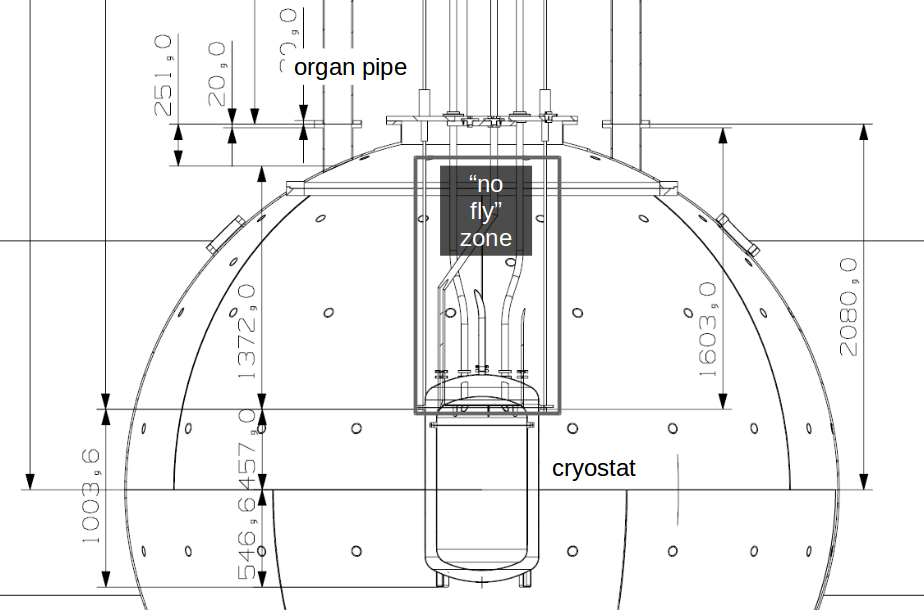
\includegraphics[scale=0.5]{Figures/NoFlyZone.png}
  \caption{``No fly'' zone for the CALIS source arm.}
  \label{fig:NoFlyZone}
\end{figure} 

\subsubsection{Default configuration}
By default the deployment device has been deployed with the longest arm (62 cm), at the center of the active volume of the TPC, with the arm rotated in the XY plane until contact with the cryostat has been made. Further details are provided in Sec.~\ref{sec:CalibCampaigns}.

Other degrees of freedom could involve shorter arm lengths, while longer arm lengths have been discussed but would require hardware modifications to the deployment device. Out of a total of four organ pipes a second one would be available for source calibration. A change in organ pipe would require a bigger effort involving also the crane in order to dismount CALIS and reinstall it on the other organ pipe. The remaining two pipes are too close to the cryo tower or reserved for the SABRE experiment \cite{SABRE}.

Finally CALIS is designed to house also a different deployment device, such as currently being planned for the neutron gun \cite{???}.
\section{Testing, Cleaning and Commissioning} \label{sec:Testing}\label{sec:Commissioning}
Testing of CALIS has been performed at FNAL in the second half of August and first half of September 2014. CALIS was installed in a building with the high bay, on a high platform, so that the full length deployment tests could be performed. The tests are repeated at LNGS prior to cleaning the system, and some validation tests are foreseen at the time of installation in CRH.  Several different tests have been conducted:
\begin{itemize}


\item{Light covers on the view ports}
Light tightness of the whole system

All viewports have  very tightly fitting covers. Additionally, the main viewport cover will additionally be held in place with clamps to avoid any possibility of accidently exposing the LSV to excessive amount of light. 



 \item{Motor controls debugging}

    LabView interface with the motor controls has been verified and responds to all commands (starting/stopping of vertical deployment) as expected.  Motor current can be read from the GUI and shows opposite signs if motor is rotating in one vs the other direction as an additional sign of the  motion direction.

\item{\bf Vertical (z) position accuracy and repeatability}
{\bf Procedure:} As a first step in testing the reproducibility of the z position as a function of step position,
a baseline relationship between step number and vertical displacement was determined. First, the distance
from the floor to the bottom of the pig was measured using a laser ranger, starting from what was found
to be the lowest pig position (fully deployed). The bottom of the pig was covered with tape to serve as a
target for the laser ranger. After this first measurement, the pig was raised, stopping approximately once
every minute to record the step position and measure the corresponding z distance, until it reached the home position (fully retracted). Subsequently, in the following test runs, the pig was again sent to each of these steps, the z position was measured with the laser ranger, and all values recorded. After 2 runs in which every step which had been recorded in the baseline was measured, it was realized that recording so many data points would require several weeks to complete the testing. The number of data points was then cut in half for 4 runs, and cut in half again for the remaining 24 runs for a total of 31 runs.

{\bf Results:} The vertical displacement of the pig was found to be extremely consistent, with no apparent
drift due to slippage or any other effect. The average uncertainty of each z coordinate was found to range
between 1-2\,mm, numbers consistent with the uncertainty of the laser ranger and the unevenness of the tape on the bottom of the pig. Fig.~\ref{fig:z_test} shows the correspondence between the z position and stepper motor count exibiting a smooth function with no visible variation of the points from the fit. No measurable slippage of the cables or accumulated offset of the stepper motor count and z position was observed during the repeated tests.

\begin{figure}[htbp]
 \centering
 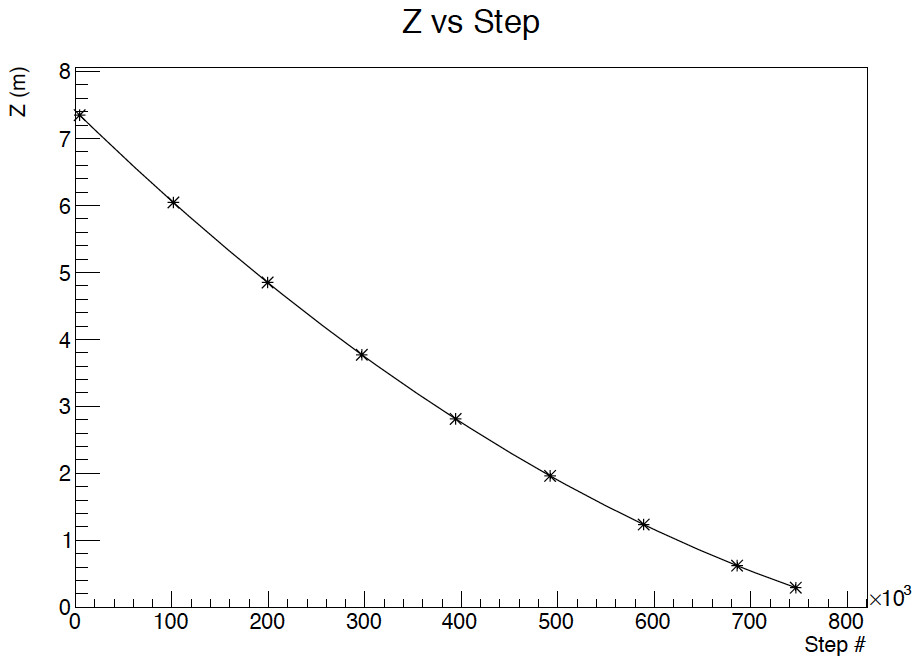
\includegraphics[width=3.2in]{Figures/Z_positioning_test}
 \caption{Plot of the z position of the pig vs the step position of the motor.}
 \label{fig:z_test}
\end{figure}


\item{\bf Lateral motion during depoyment}

The pig is deployed at a very low speed, barely visible to the naked eye. It takes about 30 minutes to deploy the system from its home position to the level of the TPC, approximetely 7\,m below. As a result, there is a negligible level of lateral motion during vertical motion at the level of 2-3\,mm. The motor has a very slow acceleration (both positive and negative) that eliminates any visible jitter at the beginning or at the end of the motion.

\item{\bf Articulation tests}

{\bf Procedure:} Arm is articulated using a manually operated hand wheel.  The arm is articulated to 90$^{\circ}$ every time. This corresponds to a different reading of the dial connected to the hand wheel for different z-position. The second calibration table required, gives correspondence between the z height and required reading on the dial to articulate to 90$^{\circ}$. 

In order to verify the consistency of articulating to the same rotation angle of 90$^{\circ}$ at all needed positions,  full articulation of the arm at different z positions was tested. For this test at Fermi lab, two vertical positions were chosen: one approximately at the center of the cryostat mock-up, and one at the lowest known position of the pig. At each position, the arm was articulated and
the required angle recorded. In order to ensure that the arm was fully articulated, a level was placed on the
arm and required to be horizontal. Additionally, the vertical displacement of the pig was measured before articulating the arm, while the arm was articulated and after the arm was again vertical. Between runs, the
pig was sent all the way back to the home position to simulate the actual deployment conditions as closely as possible. The process was repeated 10 times  (10 runs) to check consistency of articulation among independent runs.

{\bf Results:} During driving the pig up and down through the whole length of the cable, it was noticed that the arm did not return to a perfectly vertical position, which was especially noticeable when the pig was in the home position. To document this, photos were taken each time the arm was de-articulated and when it was in the home position. The hand wheel was renormalized to zero several times, but this offset continued to reappear. It did not seem to progress, however, and remained at approximately the same angle, as can be seen from the photographs in Fig.~\ref{fig:art_offset1}, Fig.~\ref{fig:art_offset2}, Fig.~\ref{fig:art_offset3} and Fig.~\ref{fig:art_offset4}. In all tested cases, offset was relatively small and did not create a problem for retracting the pig inside the lower assembly pipe and to the home posiiton. 

 It was noted that some of this offset was due to the fact that the pig is allowed to swing freely. When articulating the arm, one cable on one side of the pig is raised. This causes the pig to also slightly move in the direction of the articulation. After the
arm is dearticulated, the arm returned to vertical according to the hand wheel, but not according to visual
inspection and use of a level. Part of the offset is because the pig moved in the direction of articulation and
during dearticulation it did not return to its original position. It seemd to get stuck at a slight offset, but a
small tap on the side of the pig returned it to its original position. Additionally, the full arm articulation did
not occur at exactly the same angle each time. This was most noticeable in the lowest pig position, which
had an uncertainty of $\pm$2$^{\circ}$ (as measured on the hand crank). While searching for the cause of
this, it was discovered that a portion of the cable had been stretched during earlier load testing (cable was put under 300\,kg load to test the strengh of the crimp connections), which may have
led to a slightly uneven extension / retraction of the cables, as well as tension at certain points along the
line. The cable was unwound from the spool and allowed to return to its original length.
 The source arm had less of an offset in the vertical position than it had before adjusting the cable, although it was not perfectly straight. The articulation angle as read on the hand crank remained approximately the
same. This test will be completely repeated at LNGS with the final length of the cable in question.

\begin{figure}[htbp]
 \centering
 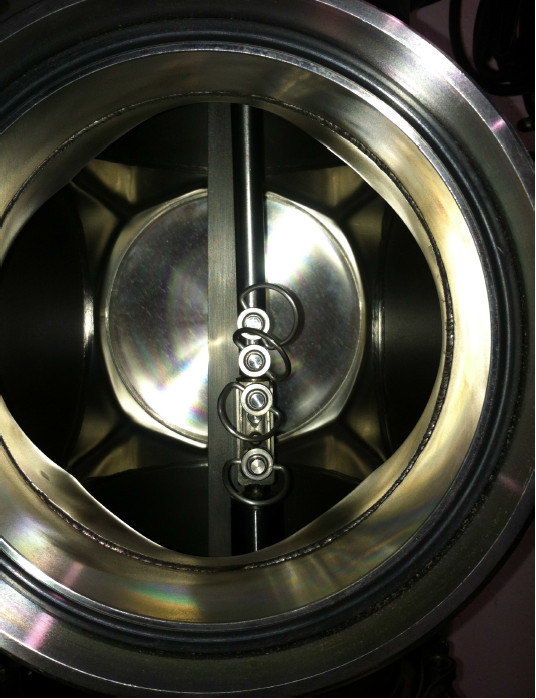
\includegraphics[width=3.2in]{Figures/ArticulationOffset1.jpg}
 \caption{Image of the pig in the home position. The offset of the arm is clearly visible, but below the level that creates problem for motion inside the organ pipe.}
 \label{fig:art_offset1}
\end{figure}

\begin{figure}[htbp]
 \centering
 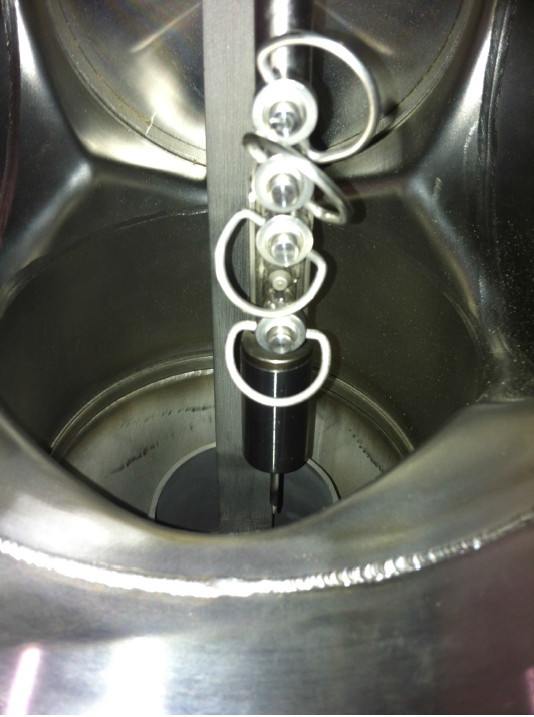
\includegraphics[width=5in]{Figures/ArticulationOffset2.jpg}
 \caption{Another image of the pig in the home position, this time looking down into the lower assembly. Again, note the offset of the arm.}
 \label{fig:art_offset2}
\end{figure}

\begin{figure}[htbp]
 \centering
 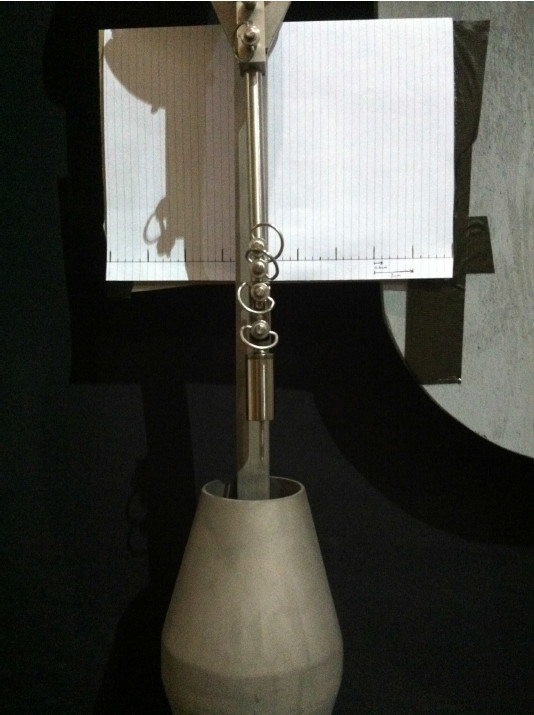
\includegraphics[width=5in]{Figures/ArticulationOffset3.jpg}
 \caption{Image of the pig next to the cryostat mock-up and the ruler used in the horizontal swing test. Note the offset of the arm.}
 \label{fig:art_offset3}
\end{figure}

\begin{figure}[htbp]
 \centering
 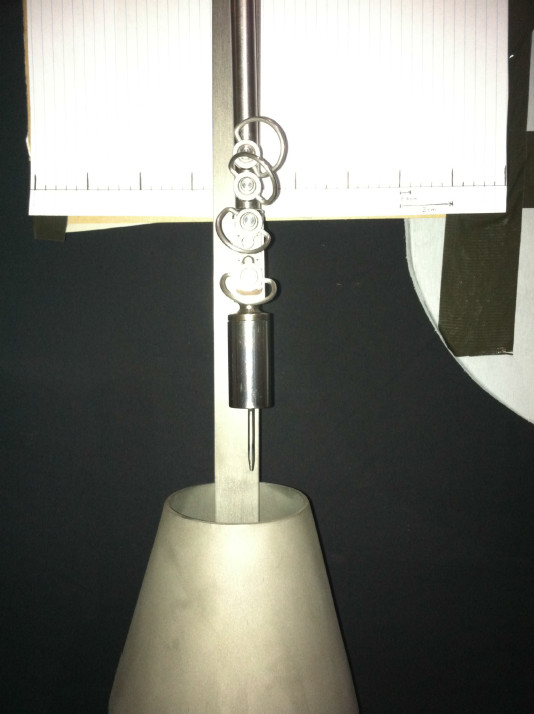
\includegraphics[width=5in]{Figures/ArticulationOffset4.jpg}
 \caption{Again, the pig next to the cryostat mock-up and ruler, a close-up of the arm offset.}
 \label{fig:art_offset4}
\end{figure}

\item{\bf Magnitude of horizontal swing during articulation}

{\bf Procedure:} To measure the horizontal swing of the system during articulation, a 'ruler' was devised and
attached to a mock-up of the cryostat, with a smallest unit of measure of 0.6 cm. The pig was then sent to
the step position where the ruler could be utilized. While the arm was articulated and de-articulated, video
was taken of the swing of the pig.

{\bf Results:}  Anaylsis of the video shows that the pig swings approximately 1.5\,cm during articulation. The articulation is very slow and the swing is very slow. It takes a couple of minutes for the arm to come to complete rest.
    
 \item{Electrical contact test for purpose of determining position of cryostat within the neutron veto}
  
\item{\bf Procedure:} One of the main goals of the first deployment of CALIS-III is to determine the location of the cryostat within the neutron veto as there is a 3-5\,cm positioning uncertainty from construction in the xy-plane and 2\,cm in the z direction.

One test to confirm the position of the cryostat is to electrically connect an arm of the pig to the cryostat. At Fermilab, the electrical contact test was simulated to prove the validity of the idea. The pig was fitted
with a special arm comprised of a stainless steel tube, and the cryostat mock-up received a stainless steel
block attached to it via screws. At the top of CALIS-III, a wire was connected between the lower assembly
and the output of a voltmeter. A wire from the stainless steel block was connected to the voltmeter input. The special arm was first articulated and then the whole assembly was rotated in the azimuthal direction in
order for the arm to make contact with the stainless steel block as can be seen in the Fig.~\ref{fig:electricalContact}.

{\bf Results:} When the arm made contact with the square, the completed circuit was indicated by the
voltmeter. Contact of the arm with the steel block was also verifed by visual inspection. The rotation and
contact was repeated several times and at each contact, the voltmeter registered (by beeping) the connection.

\begin{figure}[htbp]
 \centering
 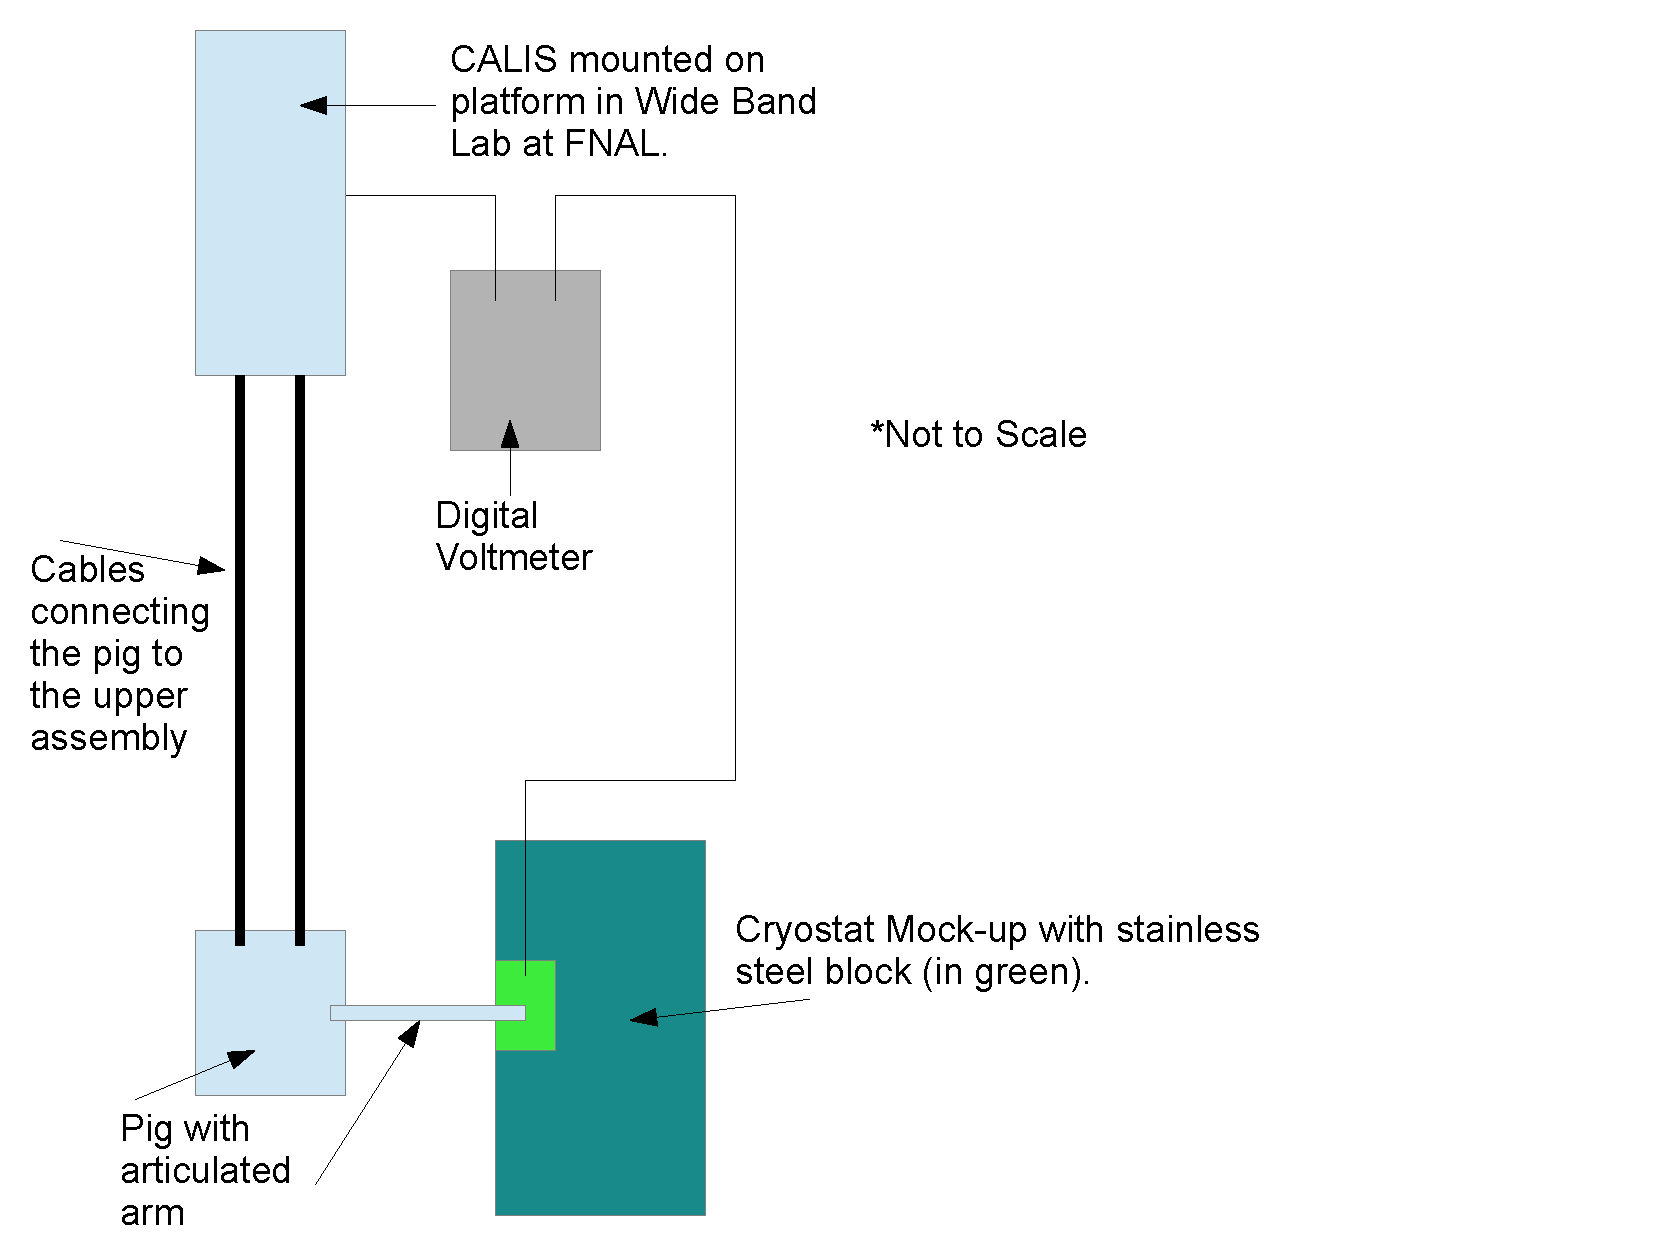
\includegraphics[width=7in]{Figures/electricalContact_FNALtest_diagram}
 \caption{Diagram of the electrical contact test performed at FNAL.}
 \label{fig:electricalContact}
\end{figure}

\item{\bf Functionality of the safety features}

Both the upper limit switch and the arm retraction switch have been tested and operated as expected. 
\begin{itemize}
\item
The pig did not move above the home position, despite the command to move up in z as the power was cut to the motor. 
\item
No z-movement was possible prior to retraction of the arm to the vertical position by the hand wheel. We verify that the arm is vertical by verifying that the dial on the protractor next to the hand wheel is pointing at zero mark. 
\end{itemize}
   
 \item{Test Ease and Accuracy of Azimuthal Rotation}
  
{\bf Procedure:} The upper and lower assemblies of CALIS-III can be rotated in the azimuthal direction.  This rotation allows the source arm to move in the xy plane for the purpose of locating the position of the cryostat within the neutron veto.  The rotation needs to be fairly easy to perform and we need to know what kind of precision and accuracy we will have. The rotation of the upper assembly requires one to loosen the clamp between the upper 
and
lower assembly. Once this is done, the upper assembly is manually moved/twisted on its axis in the direction
desired. To test this at Fermilab, the pig was deployed to the level of the cryostat mock-up and the arm articulated.
Then the clamp was loosened and the upper assembly rotated.

{\bf Results:} Despite its substantial weight, the upper assembly was able to be moved on its axis smoothly,
with no jerking or sticking. At the conclusion of testing, a band was axed to the lower assembly and
a pointer to the band was attached to the upper assembly. This is to measure the actual rotation of the
assembly. Due to time constraints, the rotation with the band attached was not able to be done. Therefore
further testing will need to be done at LNGS to determine the accuracy and precision of the azimuthal
rotation.  
 
\item{Helium Leak Tight Testing}
   
The device was tested to be helium leak tight at Fermilab.  
 
\end{itemize}

 \paragraph{}
  A full summary, along with plots, of the testing performed at Fermilab can be found in DocDB \#858.  

After the above described tests at FNAL were finished, it was concluded that \textit{\bf CALIS is in a good operating state} and is ready to be shipped to LNGS for commissioning and calibration.


\subsection{Commisioning and testing at LNGS}

 The system was shipped sub-assembled to LNGS and arrived in mid-September. Once it arrived, CALIS III was inspected and reasembled. Two rounds of tests are part of the commissioning of CALIS at LNGS: dry tests prior to cleaning and a subset of tests after cleaning the system and prior to installation on the gate valve of CRH. While the goal of the Fermi lab tests was to establish that CALIS is operating as expeced and that all designed safety features are operational, a  goal of the LNGS tests is the final characterization of CALIS to establish the absolute positioning precison of the source. 

The testing location chosen at LNGS allowed full deployment length tests and direct access to both the top of the system where the controls are and to the pig. The chosen locaiton was a tall stairway on the left side of the OPERA detector that has a platform on the fourth floor where CALIS was mounted. A movable platform accessible from the lab floor level was used to raise up to the level of the pig for all planned measurements.   The same set of tests as described above, and a few additional once related to the absolute positioning uncertainty,  have been underway.

 Final characterization of the source positioning must be done with the new cables that have been put on CALIS. The length of the cables was chosen to allow maximum safe, deployment depth that makes any contact with PMTs impossible (according to the engineering drawings of the DarkSide detectors).   Once all dry runs are performed to satisfaction, we will disassemble and clean all components in CR1 as per the normal detector cleaning procedure. After cleaning, the device will be partially assembled and moved into CRH. A subset of validation tests will be conducted from the crane in the CRH and then CALIS will be installed on the top of one of the ate valves.

\subsubsection{Dry Tests to Perform at LNGS Prior to Cleaning}
All the tests performed at Fermilab are  repeated at LNGS, but the number of runs is reduced as we do not expect to see change in the performance of the motor or the cables. While the tests at Fermi lab confirmed good operational performance of the system, the tests conducted at LNGS are calibration tests whose goal is to make the most precise prediction of the source position during deployment and establish expected uncertainty of that position.  Below is the full list of tests underway at LNGS.

 \begin{itemize}
  \item{Characterization of CALIS-III Positioning} 
 
   The CALIS-III positioning has been characterized with the final cables length. There are two components of the positioning: 

\begin{itemize}
\item
This includes the pig z position as a function of step position.
\item 
The arm 90 degree articulation point as a function of vertical pig position.  
\end{itemize}
This is necessary because, as the cable winds around the spool, the winding radius changes, increasing as the pig is lifted and decreasing as it is lowered.  This means that there is not a linear correspondence between the number of steps and the length of cable deployed.  Additionally, this non-linear dependency causes the amount of rotation required by the hand wheel for full articulation of the source arm to change as a function of the length of cable deployed.     
 
  \paragraph{}
  Every 10,000 steps (order of 10\,cm), we stop the pig and record the z position with the laser ranger, as done during the position reproducibility test at Fermilab.  The arm will then be rotated to 90$^{\circ}$ and the hand wheel position noted for the relevant z locations. The step position for key source locations commonly used during calibration will be determined, including the TPC center, 15 cm above and below the TPC center, and the cryostat top and bottom.  Once these positions have been verified by inputting the step location and measuring the z position and corresponding hand wheel rotation, the results will be formatted for easy use by CALIS-III operators.   
  
\item 
Measure the exact distance of the forward motion (in the direction of articulation) at relevant z positions, as it determins the final distance of the source to the TPC.

\item
Measure if there is any lateral change (in the azimuthal plane) when the arm is articulated at relevant z positions. While none has been observed in the previous tests, it is important to verify this in repeated deployments and articulations.

\item 
Validate the distance that the pig moves up during articulation (measured to be 10\,cm in tests at Fermilab) and verify that this number does not change between repeated articulations.

  \item
Test the arm retraction switch to confirm that the pig cannot be retracted to its home position if the arm is articulated.
  
  \item
During articulation measure the level of the horizontal swing. Confirm it to agree with Fermilab testing.
 
  \item{Determine the time it takes for the arm to reach a stable (non-moving) condition after articulation.}
 
  \item{Test the absolute encoder before and after power failure.}
  \item{Test nitrogen and vacuum systems. Measure the amount of time to evacuate the device and purge with nitrogen.}
  \item{Leak check of upper and lower assemblies.}
  \item{Reproducibility of position in x, y, and z following the full procedure.}
 \end{itemize}
 
\subsubsection{Tests to be Performed at LNGS after Cleaning}
 After cleaning of the system, we will attach CALIS-III to a crane either in CR1 or CRH to perform a reduced set of tests.  The goal is to confirm that results from tests prior to cleaning and from after cleaning match. 
  
 
  
\subsection{Proposed Commissioning Plan} \label{Proposed Commissioning Plan}
 \paragraph{}
  Detailed, step by step commissioning procedure is outlined in DocDB\#1021-v1. 
%Once CALIS is installed in CRH, we will need to test gas tightness, light tightness, and evacuation with the vacuum pump.  We will want to move the motors a little bit without opening the gate valve to ensure that all is moving satisfactorily.  Rotation of the whole assembly should be tried at this point and then an alignment will be performed.  We want CALIS to be aligned so that when the arm is articulated it is pointed towards the center of the TPC.  Next, we will open the gate valve and make sure that we can maintain the pressure as it was prior to opening the gate valve.  After that, we will proceed with a 'dummy' deployment (no source in the source holder) down through the organ pipe.  We will start with a low speed and monitor the pressure changes stopping every 5-10 cm to assess the situation.  If all systems are well, then we can increase our descent speed.  At the point of entry into the neutron veto, then we will retract the pig to home position. Once the pig reaches home position, we will again deploy into the neutron veto and attempt articulation of the arm.  We will do the first articulation when we are in optimal viewing from the cameras.  The cameras will be an extra check to ensure that we are at the position that we think we are and be sure we are not going to hit anything.  Once verified, we will dearticulate and continue the deployment, then articulate again when we are near the cryostat and desired testing position.  We will dearticulate and go back to the home position once we are satisfied that the articulation and dearticulation is complete.  As we are lowering CALIS, the DAQ will be monitored to see if there are any electronic noise problems.  We will also monitor to the PMT scalar rates.  By monitoring both the DAQ and the PMT scalars we will be able to tell if there are any light leaks.  
Once all preliminary deployments are completed, we will continue with the cryostat positioning and calibration campaign as outlined in DocDB \#977 for the neutron campaign, DocDB \#978 for the gamma campaign, and DocDB \#960 -- a spreadsheet dedicated to the full campaign.  




\subsection{Source arms}


\textit{My impression is that a drawing to scale with the cryostat, the TPCthe organ pipe and the source arm would be good here}

For articulation, there is currently a choice of three arm lengths---40.31\,cm,  57.15\,cm and 62\,cm.  

Drawing of the arm with the 


Each of these lengths are measured from the center line of the organ pipe to the end of the source holder.  The arm lengths, 57.15\,cm and 62\,cm are intentionally made too long as they will be used to determine the exact location of the cryostat; some uncertainty in the cryostat's z and lateral position exist at the level of 3 - 4\,cm. The organ pipe we intend to use is 81\,cm distant from the cryostat center (and the geometric center of the LSV sphere) as measured from the center line of the organ pipe. The cryostat is 32\,cm in radius, which leaves a distance of $\sim$49\,cm to be reached  by the arm.  The articulation of the arm is operated via a hand wheel located on the side of the upper assembly close to the top.  By rotating the hand wheel, one of the cable spools inside the upper assembly will rotate which pulls up on one of the cables attached to the pig and shortens it for the length equal to the one quarter of the gear curcamference (which is 10\,cm).  As a result, the chain at the bottom of the cables engages the articulation gear (see Fig. \ref{fig:sourcePod_arrows} for an image of the articulation gear) on the pig and raises the arm to horizontal.  The chain has a guard rail that ensures that chain can never come of the gear. Thus, in the process of articulation the entire pig along with the source arm shifts up for 10\,cm.  See Fig. \ref{fig:pigAndCables_fullView} and  Fig. \ref{fig:sourceArmRotation} for a closer look at how CALIS III articulates the arm. In order to determine the degree of articulation of the arm, a protractor is placed next to the hand wheel.  This protractor and the hand wheel are calibrated together for an accurate reading of the articulation. The reading of the protractor dial is different at different heights and calibration table obtained from the tests is used to determine the dial setting necessary to articulate the arm to horizontal position. We have adopted a spherical coordinate system for the rotation of the system and the articulation.  Articulation of the arm is measured in $\theta$ from the z-axis; when the arm is fully articulated, it is at 90$^{\circ}$ and when it is in its vertical position it is at 180$^{\circ}$.  As mentioned in Sec. \ref{The Lower Assembly}, the rotation of CALIS III is done in the xy-plane which corresponds to the azimuthal direction, a rotation in $\phi$.  See Fig. \ref{fig:coordinate_system} for details. 


%%%%%%%%%%%%%%%%%%%%%%%%%%%%%%%%%%%%
\subsection{Calibration of Z-position and Articulation Angle}  
%%part of testing, cleaning and commissioning section

\subsection{Operational Procedure}
After the testing and commissioning CALIS has been installed inside CRH... 

Well, there also have been test deployments before that.
\subsubsection{Source Insertion}

\subsubsection{3 special positions}
home position or parking position - gate valve closed. The 

center of the TPC.

Full extension position - length of the cable.






\paragraph{Opening the Gate Valve}
\subsubsection{Positioning of Source}
\paragraph{Contact with Cryostat}
\paragraph{Cameras}
\subsubsection{Source Retraction and Extraction}
The source may not get in contact with the liquid scintillator. It is therefore sealed during the deployment in a dedicated source holder. In order to exchange sources the source arm and source holder has to be extracted from the pig into CRH and thereby comes in contact with normal air, containing oxygen and traces of water. After insertion a flush \& purge cycle is used to reduce, as known from glove boxes. No glove box present. Much more compact design.
% no glove box

After each deployment check that there is no leakage of Scintillator inside the source holder.



for what is helium leak tightness necessary? What was tested for helium leak tightness.



%tested for helium leak tightness

 
\section{Calibration Campaigns}\label{sec:CalibCampaigns}
\subsection{Radioactive Sources}
For calibration of \lsv\ detector response and \tpc's response to electron recoils (ER) $^{57}$Co, $^{133}$Ba and $^{137}$Cs were selected. $^{22}$Na was deployed in a later calibration campaign. They allow a cross-calibration with $^{83m}$Kr injected in Argon recirculation system during dedicated campaigns and internal $^{39}$Ar, as they cover the $^{39}$Ar energy range (see also Table~\ref{tbl:GammaSources} and Fig.~\ref{fig:GammaSources_Ar39spectrum}). %As the interaction length increases with energy in LAr, the different gamma sources allow also to probe different regions of the TPC active volume.  

After a gamma source energies preselection, detailed studies with DarkSide Monte Carlo simulation package G4DS \cite{DS50:G4DS:paper} were performed to select appropriate source activities and check various deployment positions' feasibility and physics reach. Sources with suitable activities were identified for deployment considering also constraints from \lsv\ and \tpc\ DAQs (Table~\ref{tbl:GammaSources}).

Energy variables are calibrated in photo-electrons (PE) using dedicated laser calibration runs, in which each PMT's single PE charge spectra are fitted and a PE-charge gain is determined. 
These laser runs are also an integral part of a calibration campaign requiring a laser run every few hours and at least on each change in DAQ, \tpc\ or CALIS configuration, such as drift field changes or source position changes.

\begin{figure}[htbp]
 \centering
 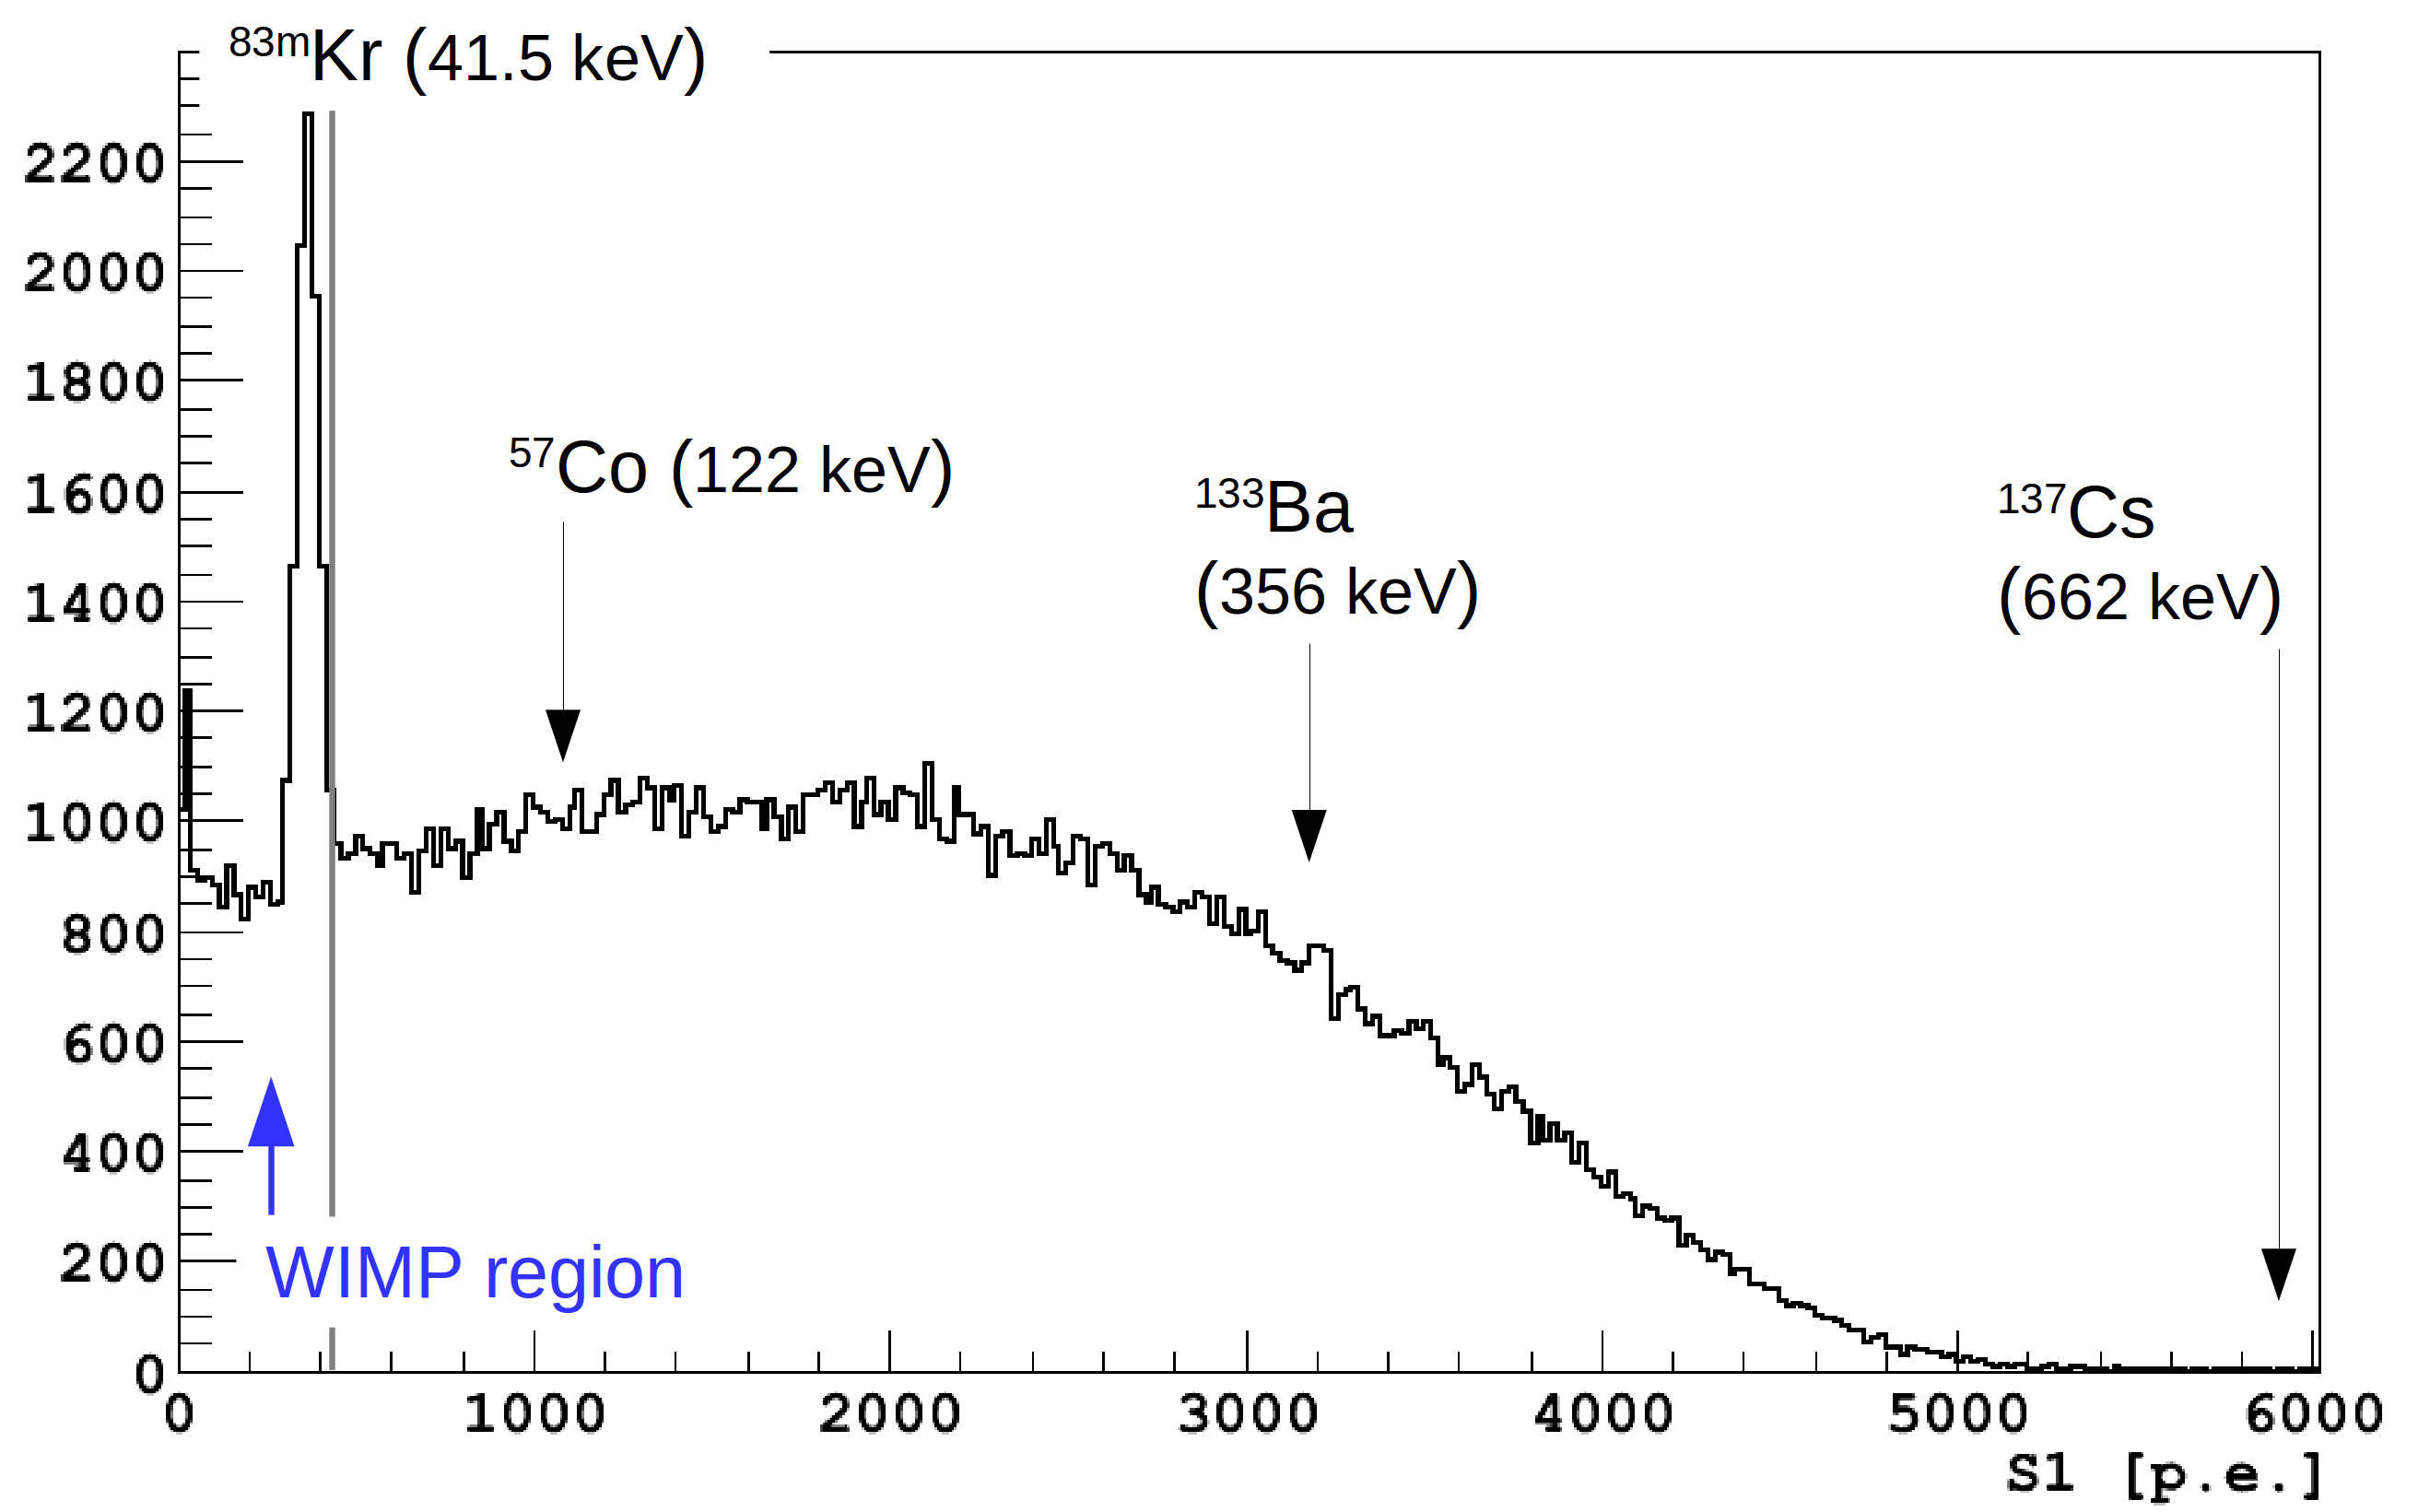
\includegraphics[width=0.8\textwidth]{Figures/GammaSources_Ar39spectrum.png}
 \caption{Scintillation spectrum (S1) at null field showing a $^{83m}$Kr peak on internal $^{39}$Ar $\beta$ spectrum. Positions of full absorption peaks of three gamma sources are indicated and cover $^{39}$Ar spectrum's full range.
\label{fig:GammaSources_Ar39spectrum}}
\end{figure}

\begin{table}[htbp]
\centering
\caption{Gamma sources deployed in DS-50, $^{39}$Ar and $83m$Kr \cite{Lippincott:2010jb}. Interaction length is in liquid Argon. $^{39}$Ar activity has been approx. 50 Hz during AAr filling and negligible in the UAr phase. The Kr source activity varied from campaign to campaign, but was in range of a few Bq to some tens of Bq.} %\cite{Lippincott:83mKr}
\centering
\begin{tabular}{|l|l|l|l|l|l|}
\hline
\textbf{source} & \textbf{type} & \textbf{energy} & \textbf{half life} & \textbf{interact. length} & \textbf{activity} \\ \hline
$^{57}$Co & $\gamma$ & 122 keV & 0.744 y & 4.4 cm & 35 kBq \\ \hline
$^{133}$Ba & $\gamma$ & 356 keV & 10.54 y & 7.5 cm & 2 kBq \\ \hline
$^{137}$Cs & $\gamma$ & 662 keV & 30.2 y & 9.5 cm & 0.65 kBq \\ \hline
$^{22}$Na & $\gamma$ & $2\cdot 511$ keV + 1274 keV & xxx y & 8.4/ 11.3 cm & 11 kBq \\ \hline\hline
$^{39}$Ar & $\beta$ &  565 keV endpoint& xxx y & sub-mm & 50 Bq (1 Bq/kg) \\ \hline
$^{83m}$Kr & 2 $\beta$ &  32.1 keV + 9.1 keV & xxx y & sub-mm & \\ \hline
\end{tabular}
\label{tbl:GammaSources}
\end{table}

\subsection{Calibration Campaigns Timeline and Stability}
Following calibration campaigns were performed between October 2014 and April 2016:
\begin{itemize}
\item First extensive campaign involving all gamma sources and both high and low activity AmBe neutron source took place in October and November 2014 at LNGS. \tpc\ was filled with Atmospheric Argon  with an inherent trigger rate of approx. 50 Hz from $^{39}$Ar. \lsv\ liquid scintillator consisted of PC only with $<0.1 \%$ TMB and 1.4 g/l PPO as wavelength shifter.
%Fig.~\ref{???} shows the different configurations in which data has been taken as a function of source energy, source position and drift field.

\item In January and February 2015 a second campaign focusing on \lsv\ calibration using low activity AmBe source was performed. Before this \lsv\ was reconstituted with 5\% TMB. Two deployments were performed at two different PPO concentrations (0.7 g/l and 1.4 g/l), allowing to study PPO concentration impact on alpha and gamma quenching. (1.4 g/l is our nominal PPO concentration, see also Fig.~\ref{fig:LSV:Calib}, right)

\item In August 2015 a $^{22}$Na source was deployed next to cryostat for TPC calibration. This was first gamma source calibration campaign after UAr deployment within \dsf.
\item In December 2015 an $^{241}$Am$^{13}$C neutron source has been deployed, allowing an in-depth study of detection efficiency of prompt neutron recoil signal in absence of correlated 4.4 MeV gamma, obfuscating neutron recoil signal in case of an AmBe source.
\end{itemize}

In dedicated analyses it has been shown that calibration campaigns have not affected negatively light yield or introduced radioactivity into the LSV \cite{Agnes:2015qyz}.

%\begin{figure}[htbp]
%\centering
%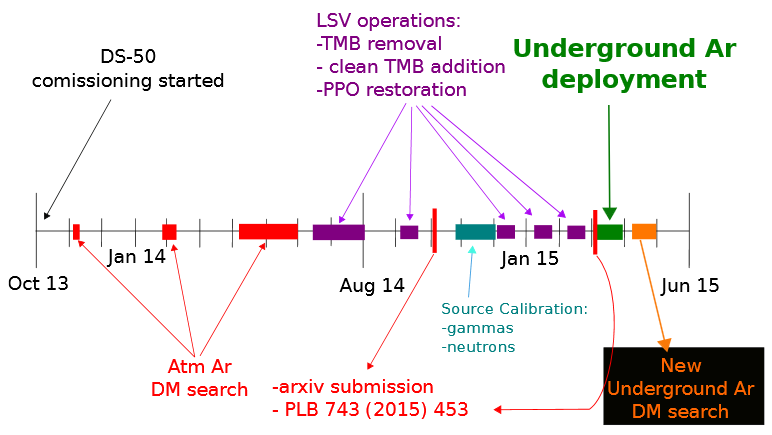
\includegraphics[width=0.7\textwidth]{./Figures/Yann_timeline.png}
%\caption{In black the stability of the LSV LY is monitored using internal $^{60}$Co emitted from the cryostat steel, in blue the stability %of the rate of radioactivity in the LSV is shown. Before and after calibration campaigns both the LY and the rate remain unaffected.
%\label{fig:LSV:Stability}}
 %\end{figure}


\subsection{TPC Calibration}
A few calibration results are shown illustrating acquired calibration data quality and their description in G4DS.

\subsubsection{$^{57}$Co S1 energy}
Fig.~\ref{fig:CalibData:Co57} shows a data-MC comparison of scintillation signal S1 spectrum of a $^{57}$Co calibration source deployed next to cryostat and close to TPC active volume center. S1 distribution is overlayed by an equivalent selection of G4DS MC simulation events.\mymarginpar{The plot is from Paolo's G4DS talk \@ DS2016, UCLA. Ideally one could get an official copy from the MC paper.}

\begin{figure}[htbp]
\centering
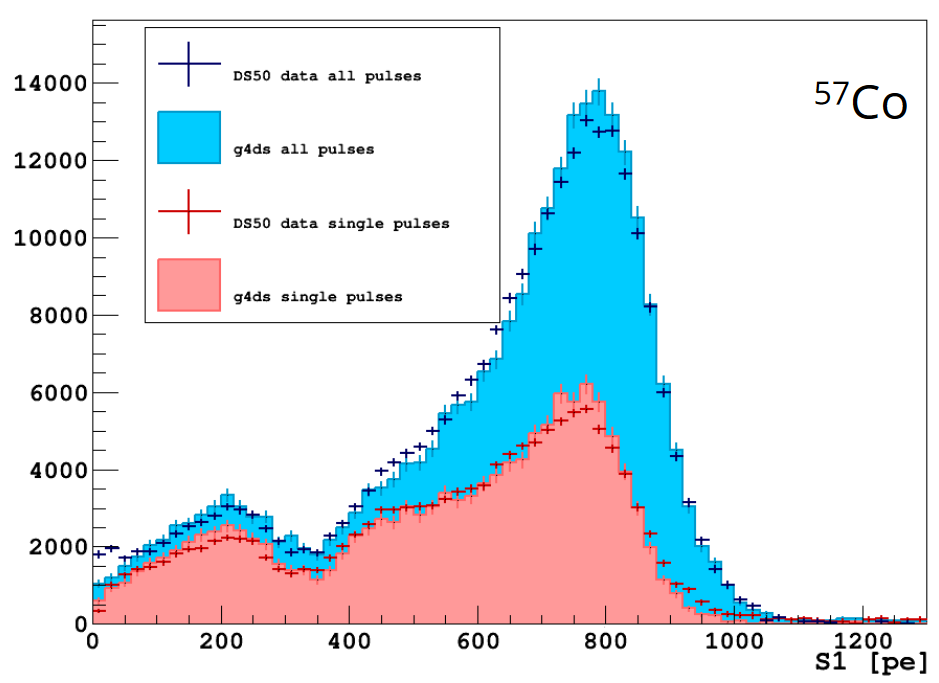
\includegraphics[width=0.7\textwidth]{./Figures/57Co_Paolo_G4DS_UCLA.png}
\caption{Data-MC comparison for $^{57}$Co source deployed next to cryostat. In magenta distribution a single-site interaction requirement is imposed as for dark matter events and for blue distribution this constraint is removed \cite{DS50:G4DS:paper}.
\label{fig:CalibData:Co57}}
 \end{figure}


\subsubsection{F90 distribution from $^{241}$Am$^9$Be neutron data}\label{sec:CalibData:NR}

Fig.~\ref{fig:CalibData:F90} shows good agreement between F90 medians and S1 spectra measured from $^{241}$Am$^9$Be neutron data and those derived from \SCENE\ measurements, which have been used to determine nuclear recoil energy scale and NR acceptance regions for WIMP dark matter search \cite{Agnes:2015gu, Agnes:2015_uar}.
\begin{figure}[htbp]
\centering
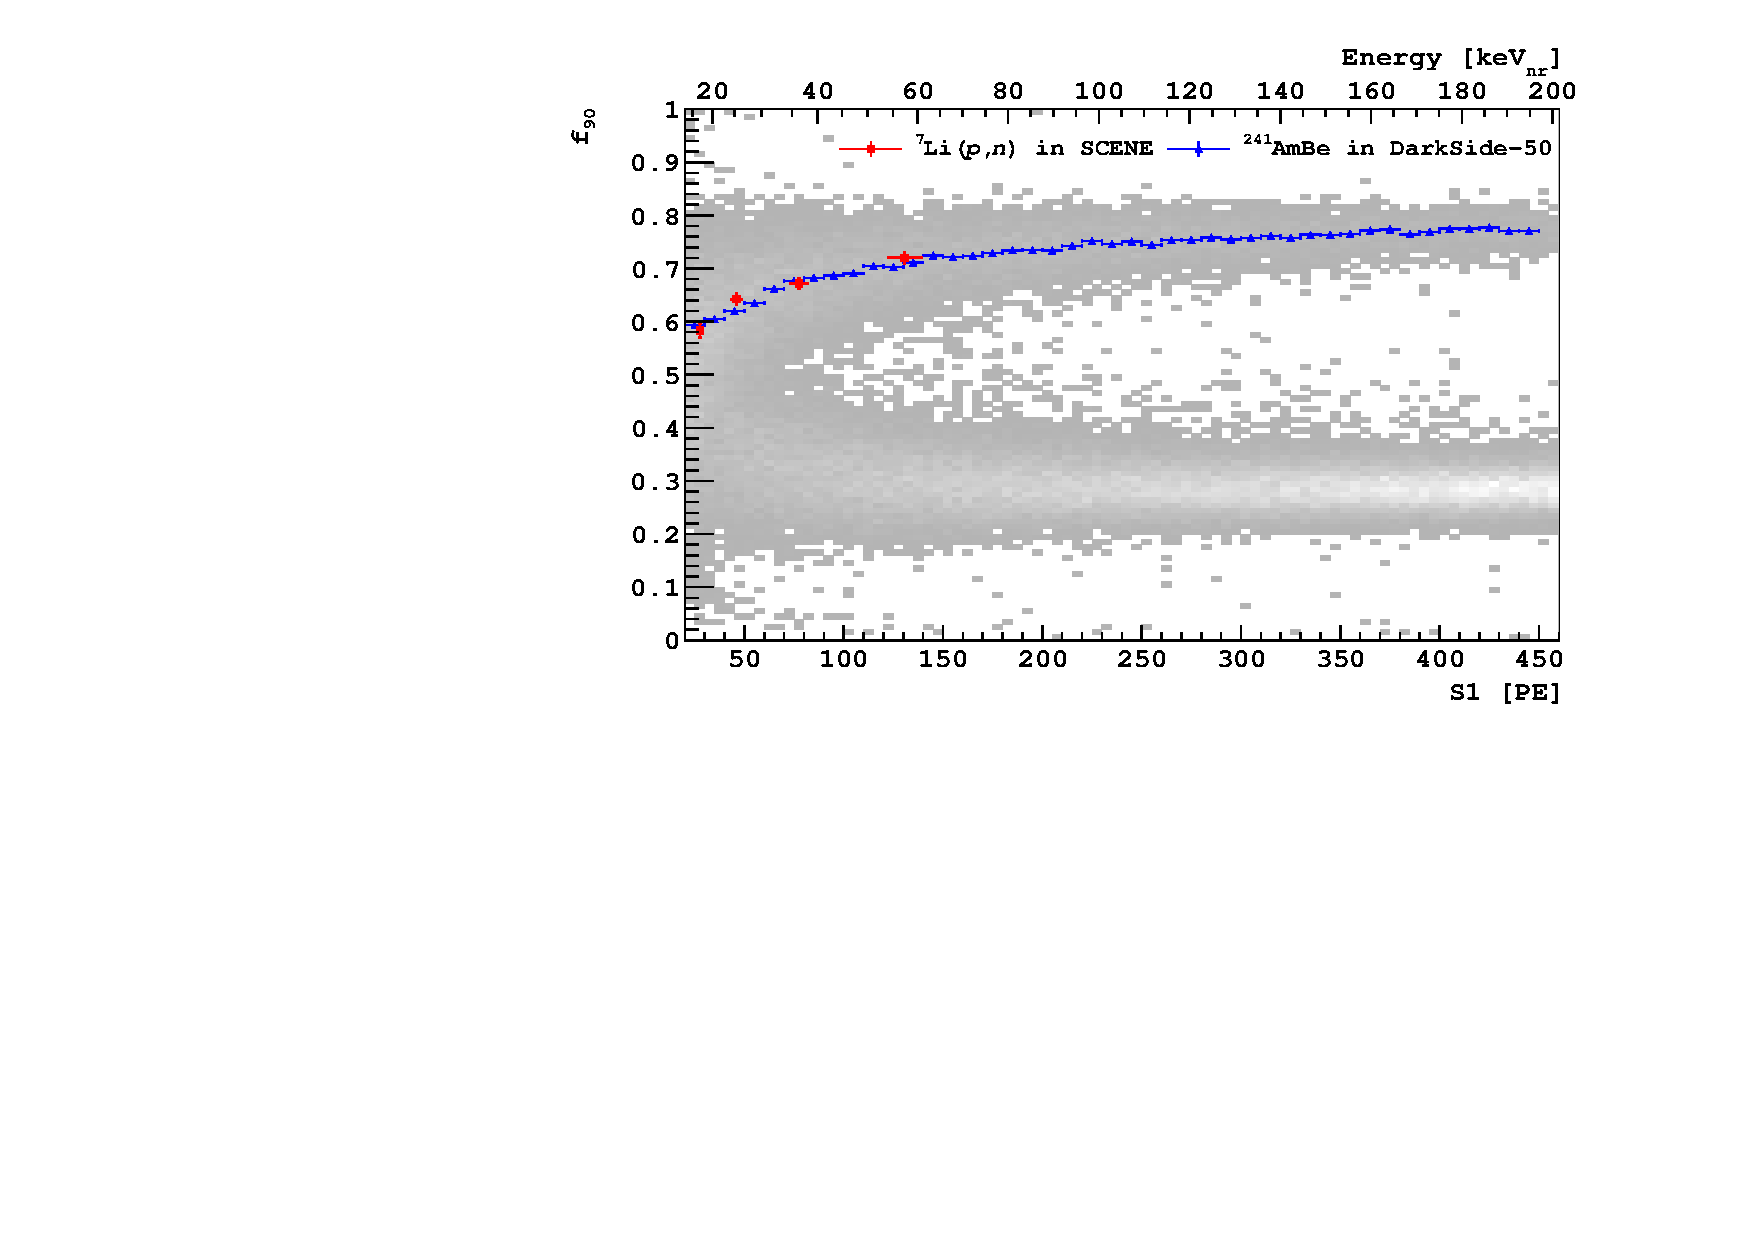
\includegraphics[width=0.7\textwidth]{./Figures/DSf-UArAmBeDMSStCut.pdf}
\caption{Plot of F90 vs. scintillation signal S1 from a high rate AmBe neutron source calibration of \dsf\ in grey, upper NR band from AmBe calibration and lower ER band from $\beta$-$\gamma$ backgrounds are visible. Overlaid are \FNinety\ \NR\ median vs. \SOne\ from a high-rate {\it in situ} AmBe\ calibration (blue) and scaled from \SCENE\ measurements (red points) \cite{Cao:2015ks}. There is very good agreement between the two.  High source intensity and correlated neutrons and $\gamma$-ray emission by AmBe source contribute events outside nuclear recoil and electron recoil bands. (reproduced from \cite{Agnes:2015_uar})\label{fig:CalibData:F90}\label{fig:DSf-UArAmBeDMS}} 
\end{figure}


\subsubsection{Source position}
Tests at LNGS established the deployment system's positioning accuracy to be about $\pm$1 cm after a 7 meter journey into the \dsf\ \lsv.
%comment to the "about $\pm ": the tilde $~ \pm$ did not show up at all in the output.
During first calibration campaign several runs have been taken with source at its central position (731000 motor step counts). Fitting t$_{drift}$ distribution at that position for a sequence of runs a systematic shift vs.~time has been observed (Fig.~\ref{fig:SourcePosition}, right). The source position has been on average 157.4 mm below the grid with an RMS of 10.1 mm. Following that observed systematic shift with time deployment procedures were revised to avoid such a time dependency in the future and to improve the deployment precision: Prior to moving source to its target position, deployment device is sent to its lowest position, where cables are fully unwound and any build-up in the cables is released. It is worth mentioning this does not induce significant uncertainties for calibration data analyses, as t$_{drift}$ distribution can be measured in-situ on a per-run basis and hence does not affect our dark matter analysis.
\begin{figure}[htbp]
\centering
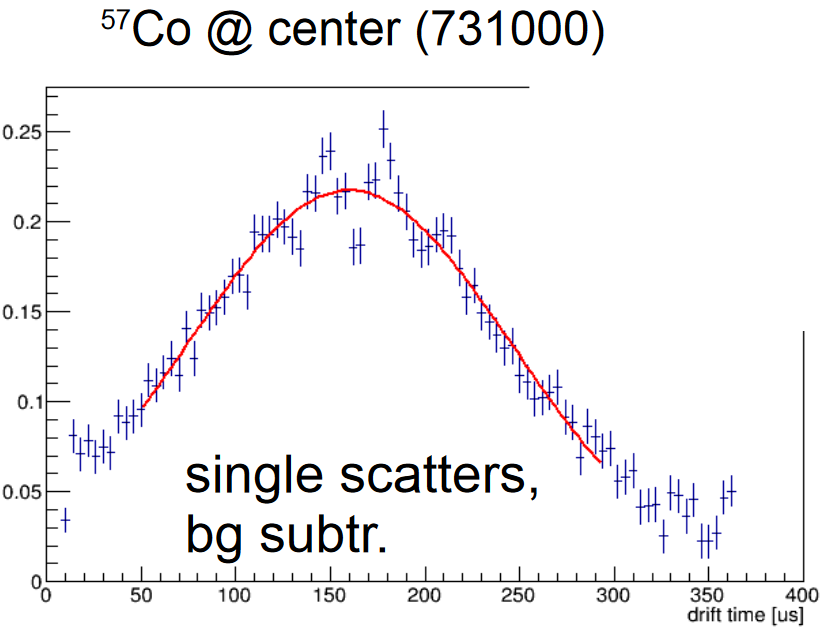
\includegraphics[width=0.48\textwidth]{./Figures/Tdrift_distribution_Co57_DocDB1288.png}
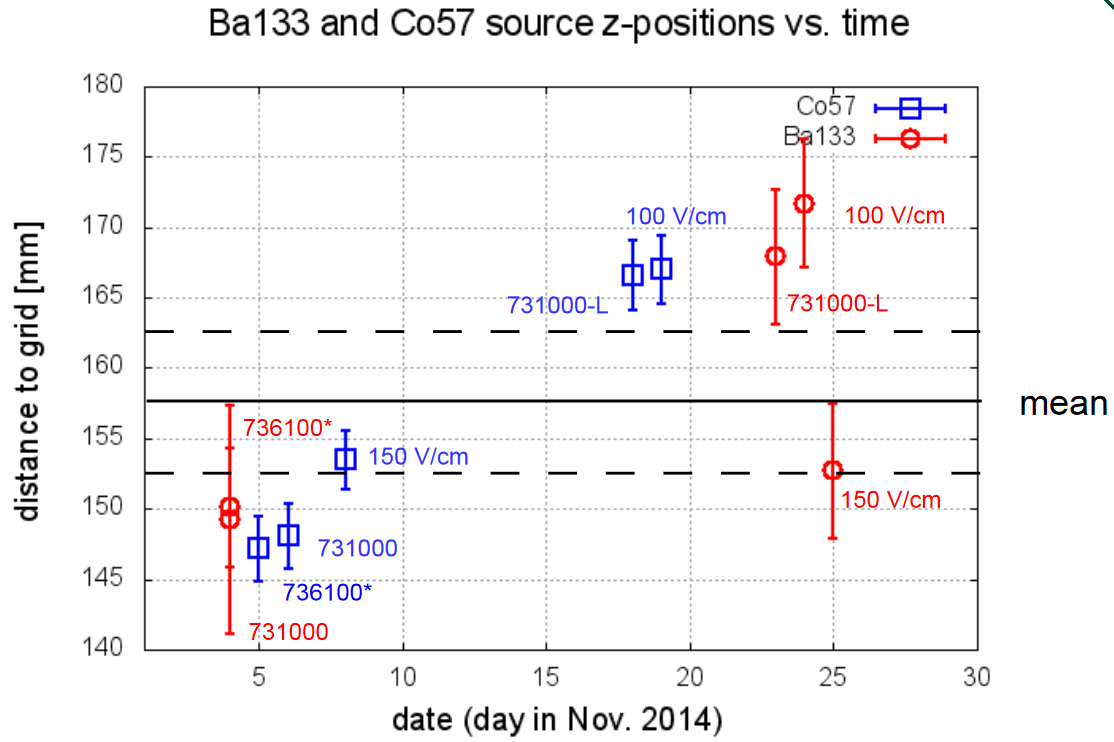
\includegraphics[width=0.48\textwidth]{./Figures/SourcePosition_vs_time_DocDB1288.png}
\caption{\textit{left:} A t$_{drift}$ distribution encoding the Z-position of $^{57}$Co deployed next to TPC vertical center.
\textit{right:} Shift of source position relative to TPC grid as a function of time when deployed to same place.
\label{fig:SourcePosition}} 
\end{figure}

For XY position azimuthal angle distribution in XY plane has been studied and a 139 degree mean was observed with a 1.2 deg RMS. (One degree corresponds to 6 mm at the outer cryostat, where source is positioned.) However an independent XY reconstruction algorithm gave 142.5 degrees with an 0.8 deg RMS, so that systematic uncertainties from reconstruction dominate over XY precision. %\cite{DS:XY:paper}.
\mymarginpar{This is from DocDB 1288. Ideally one could cite a XY paper here, which is not published yet.}


%%%%%%%%%%%%%%%%%%%%%%%%%%%%%%%%

\subsection{Liquid Scintillator Veto}\label{sec:LSV:gammasources}

In Fig.~\ref{fig:LSV:Calib} (left) a data-MC comparison of LSV charge spectra from a $^{137}$Cs source deployed in LSV next to cryostat is shown \cite{DS50:G4DS:paper}.
In January and February 2015 LSV scintillator reconstitution was completed and a second LSV calibration using AmBe neutron source was undertaken to further study various LSV neutron detection channels. With a borated scintillator, a critical aspect of neutron detection efficiency is the capability to observe \brbortenground\ capture branch leading to a \enbortengroundalpha\ $\alpha$ + $^7$Li(g.s.) without accompanying 478 keV $\gamma$-ray. As shown in Fig.~\ref{fig:LSV:Calib} (right) the de-excitation channel is clearly observed at around 30 PE.

\begin{figure}[htbp]
\centering
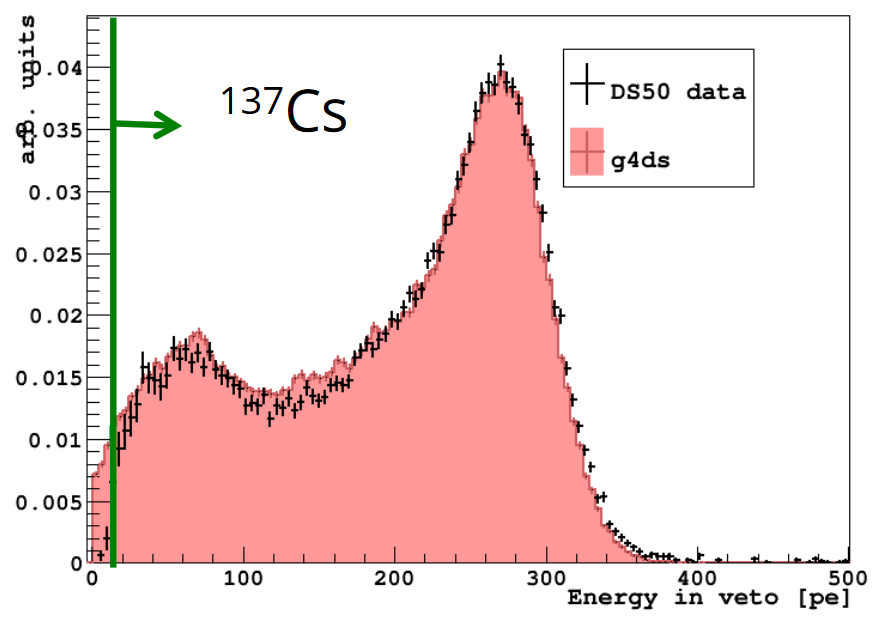
\includegraphics[width=0.48\textwidth]{./Figures/137Cs_Veto_Paolo_G4DS_UCLA.png}
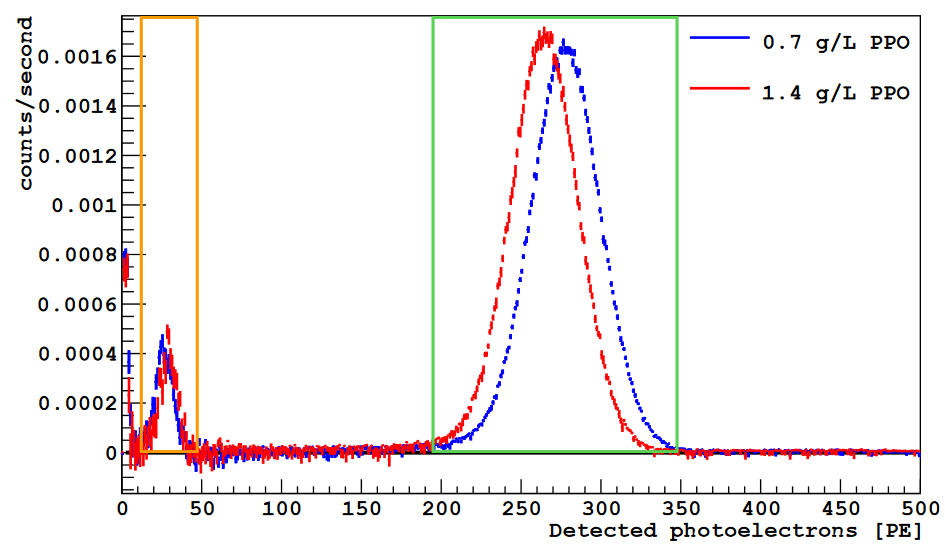
\includegraphics[width=0.48\textwidth]{./Figures/AmBe_LSV_VetoPaper.png}
\caption{\textit{left:} LSV charge spectra data-MC comparison from $^{137}$Cs source deployed in LSV next to the cryostat \cite{DS50:G4DS:paper}.
\textit{right:} Clear neutron capture signal detection on $^{10}$B in LSV leading to a \enbortengroundalpha\ $\alpha$ + $^7$Li(g.s.) at $\approx$ 30 PE (orange box). Peak on the right at $\approx$ 270 PE (green box) is from 93.6 \% of captures that lead to the $^7$Li excited state reaction, with the accompanying 478 keV-ray. The entries below 10 PE are due to PMT after-pulses. Data has been taken before and after varying PPO wavelength shifter concentration in the scintillator with the source rotated 70 cm away from the cryostat. In both cases the deexcitation to ground state is clearly observed.\cite{Agnes:2015qyz}
\label{fig:LSV:Calib}} 
\end{figure}

%%%%%%%%%%%%%%%%%%%%%%%%%%%%%%%%
%%%%%%%%%%%%%%%%%%%%%%%%%%%%%%%%
%%%%%%%%%%%%%%%%%%%%%%%%%%%%%%%%


\section{Conclusions}\label{sec:Conclusions}\label{sec:Conclusion}
CALIS is a simple and affordable, yet effective source deployment system that has been successfully used to deploy sources in LSV and next to TPC and to conduct several successful calibration campaigns. No adverse effects on the LSV or TPC have been noticed.

%summarize that the LSV and TPC detector have not been negatively affected.
%that's a sentence for the summary: The critical contribution by CALIS is the neutron veto detection efficiency calibration using dedicated neutron sources
%neutron gun inside a dedicated deployment device currently under development (Section \ref{sec:Outlook}).
%Refer to the next generation DS-detector.
%\section{Epilogue}\label{sec:Epilogue}
%here I would list all upcoming DarkSide papers and how they are in relationship with each other. Since so many papers are in preparation I would find that %helpful. Even if it is not eventually put into the paper.

%\section{Analysis}\label{sec:analysis}

\subsection{TPC}

\subsubsection{$^{57}$Co S1 energy}
Fig.~\ref{fig:CalibData:Co57} shows a comparison of the scintillation signal S1 spectrum of a $^{57}$Co calibration source data deployed next to the cryostat and close to the TPC active volume center. Overlayed is the S1 distribution from an equivalent selection of G4DS MC simulation. Besides passing basic cuts like baseline found or all electronics channels present, the events were restricted to single-site interactions having one S1 and one S2 pulse, also the $^{39}$Ar background has been subtracted statistically. In the MC instead of an electronics simulation a clustering algorithm has been applied, that groups individual energy deposits and sums up the corresponding number of PE. A single-cluster cut has been applied to correspond to single-site interactions. The $^{57}$Co gamma ray spectrum (122 keV) reaching the TPC is significantly distorted by having to pass through the stainless steel source holder, outer and inner cryostat and the copper field cage rings before reaching the TPC's active volume.  These effects are accounted for by the MC even though refinements in the material description will further improve the already encouraging data-MC agreement. 

\begin{figure}[htbp]
\centering
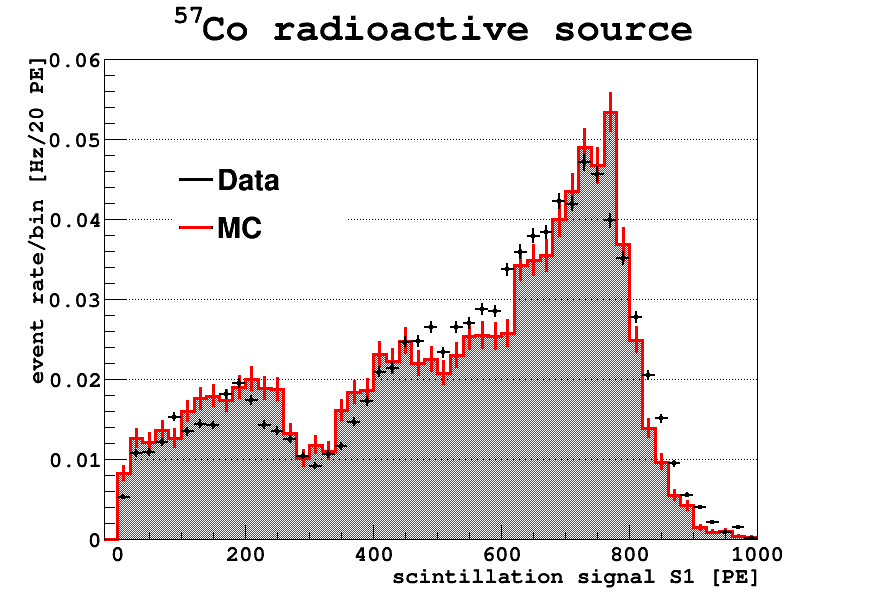
\includegraphics[width=0.6\textwidth]{./Figures/Co57_LArTPC_center.png}
\caption{Data-MC comparison for the $^{57}$Co source deployed next to the cryostat. While some improvements are yet to be made, the level of agreement between the simulation and the various complex features of the data is very encouraging.
%A lack of resolution in the MC is expected as smearing due to electronics and reconstruction effects are not taken into account in the MC. THIS DOES NOT MAKE SENSE
\label{fig:CalibData:Co57}}
 \end{figure}


\subsubsection{position distributions}
\begin{figure}[htbp]
\centering
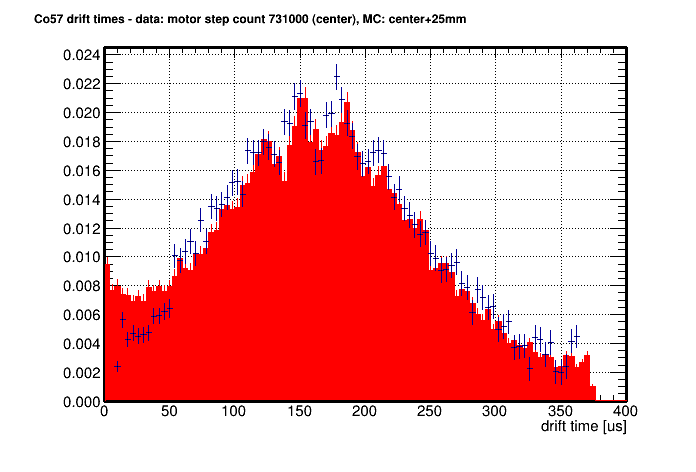
\includegraphics[width=0.55\textwidth]{./Figures/Co57_tdrift_data_731000-center+25mm.png}
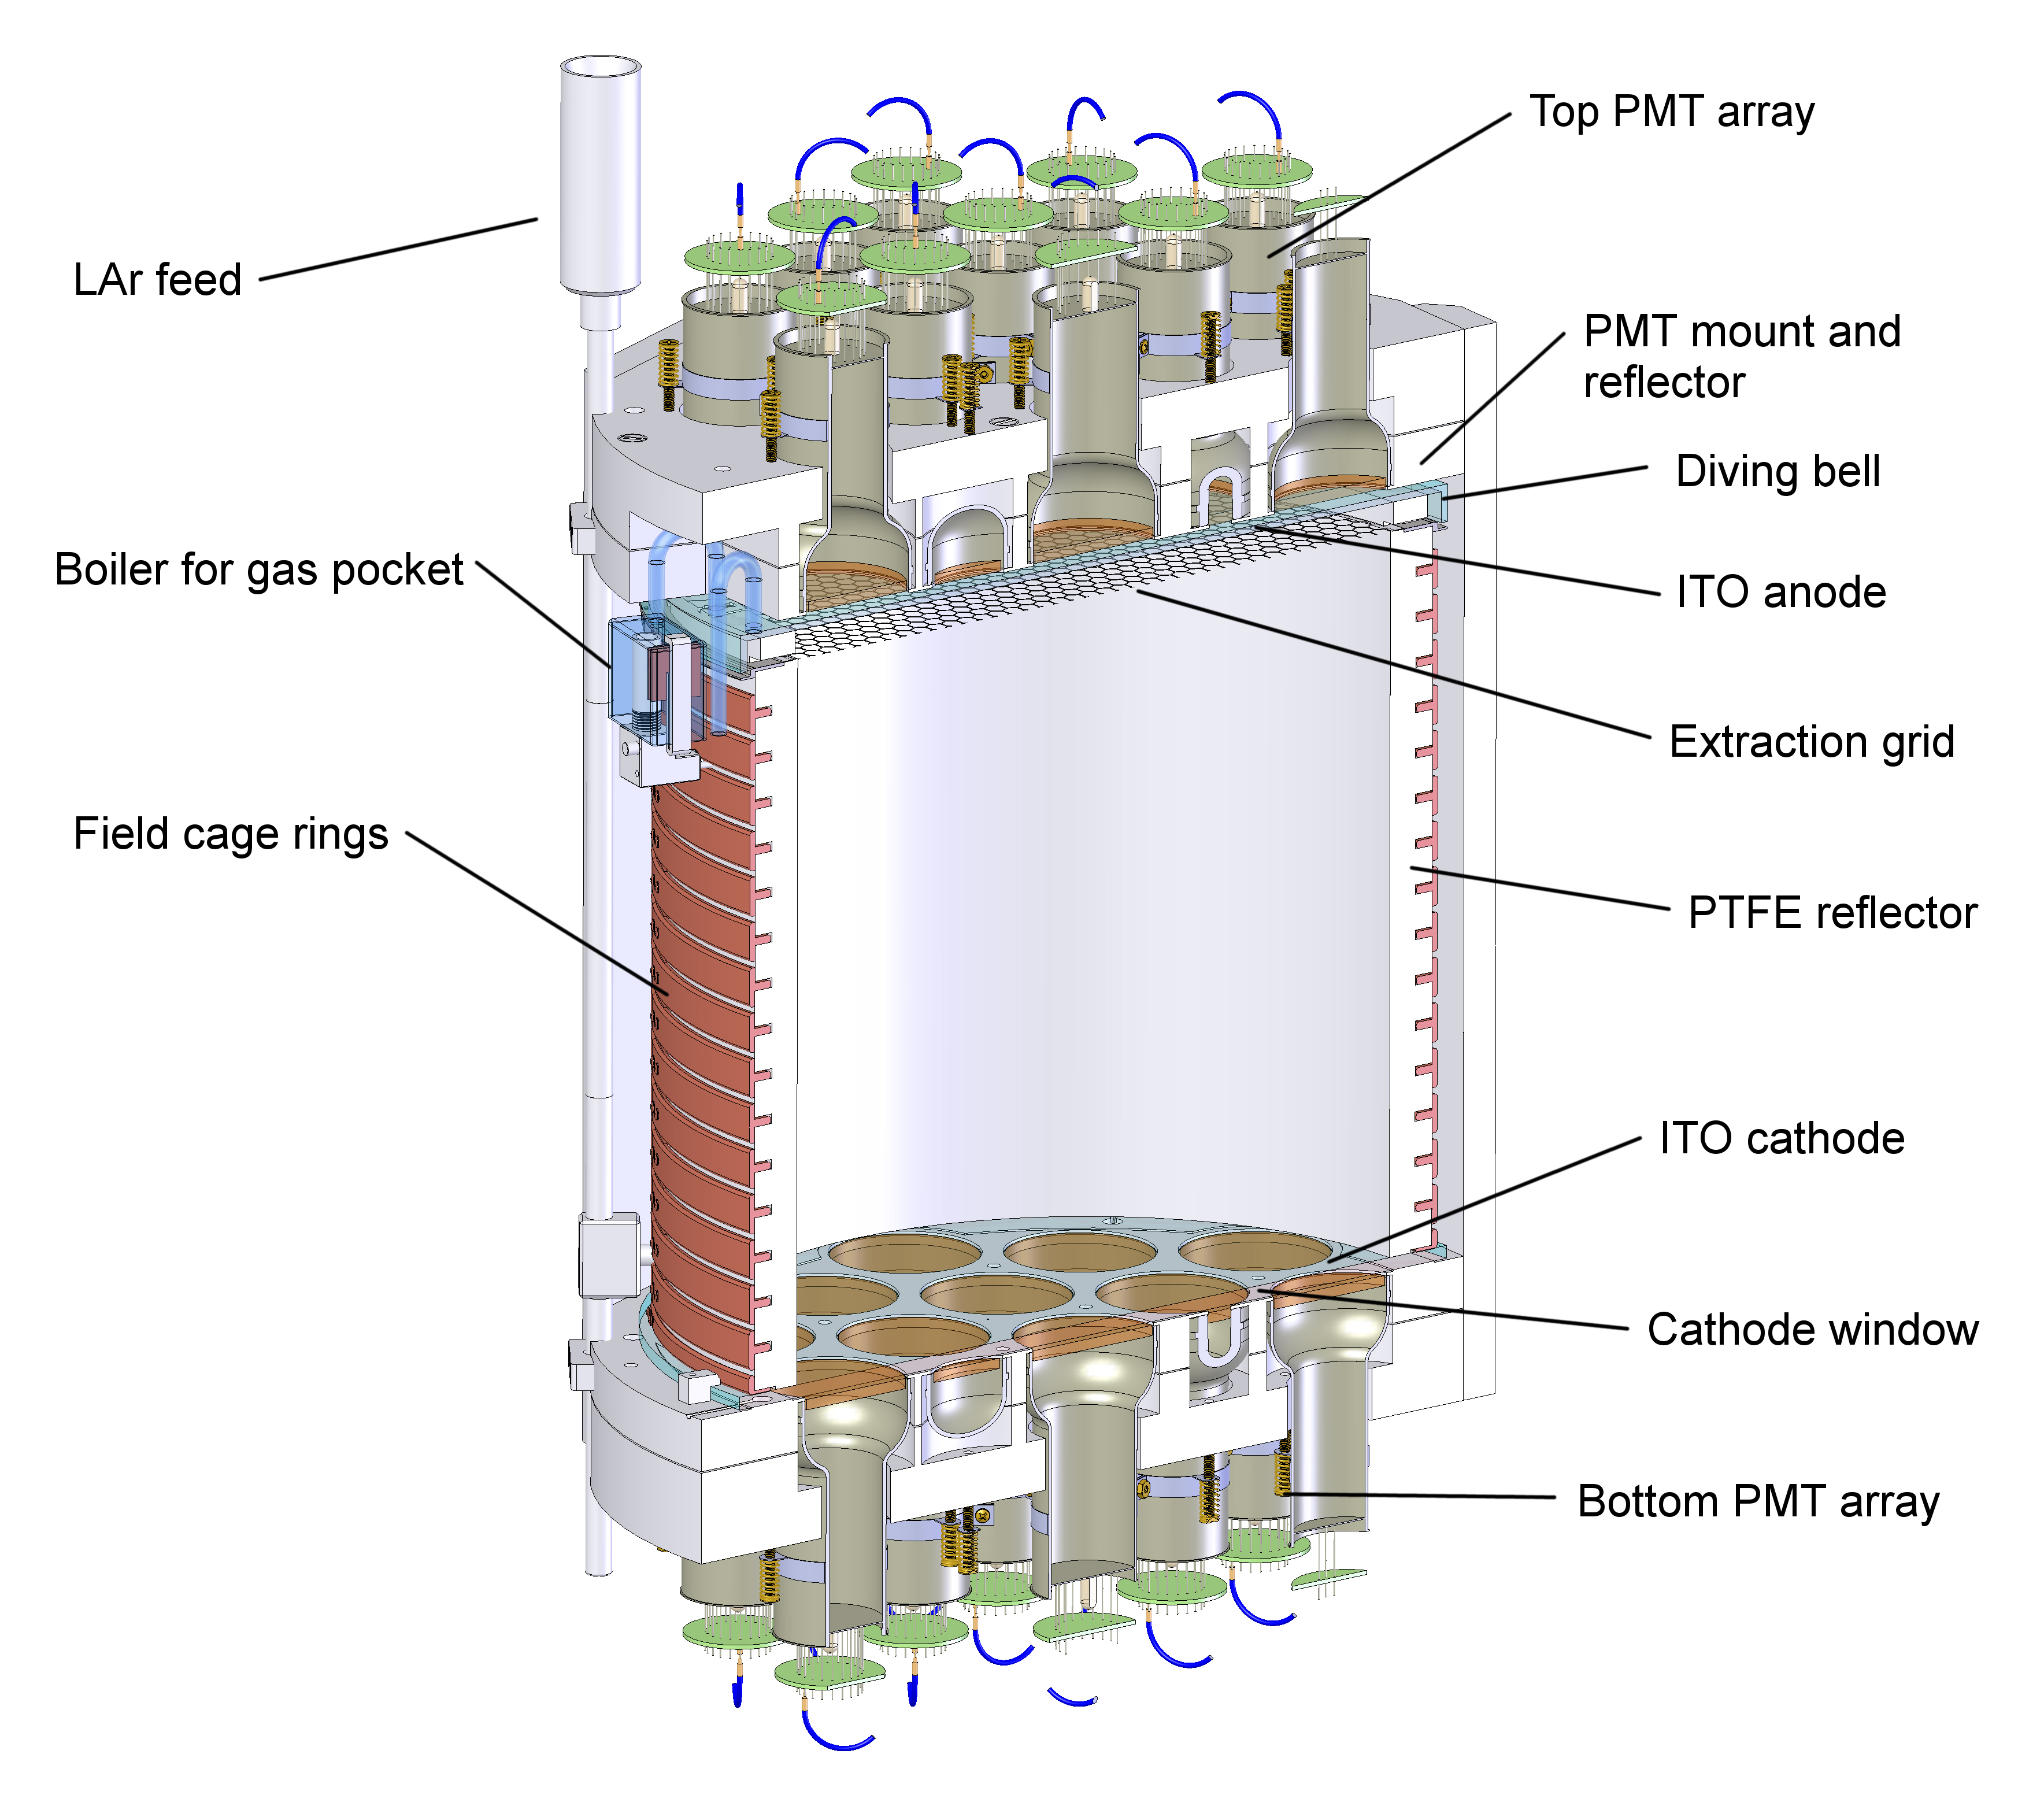
\includegraphics[width=0.43\textwidth]{./Figures/50kg_Assembly_4-1-13_section_annotated_2.JPG}
\caption{\textit{left}: Data-MC comparison for the t$_{drift}$ distribution of the $^{57}$Co source deployed next to the cryostat and close to the active volume center. 
\textit{right:} Schematics of the TPC (without inner and outer cryostat) showing in particular the field rings, that cause a characteristic wave in the t$_{drift}$ spectrum of $^{57}$Co, which is also reproduced in MC (left) \cite{DS50:first_paper}.
\label{fig:CalibData:Co57:t_drift}}
\end{figure}

The t$_{drift}$ distribution of $^{57}$Co in Fig.~\ref{fig:CalibData:Co57:t_drift} is the same run set and event selection as for the S1 spectrum in Fig.~\ref{fig:CalibData:Co57}. It nicely illustrates the impact that the field rings have on the distribution. Fig.~\ref{fig:CalibData:XY_distrib} shows XY distributions of $^{133}$Ba and $^{137}$Cs sources deployed touching the cryostat from the left and right, respectively, exemplarily out of a pool of possible XY distributions.

\begin{figure}[htbp]
\centering
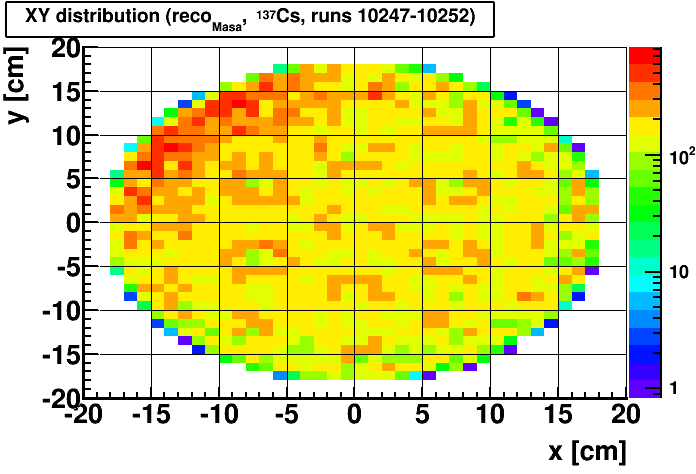
\includegraphics[width=0.55\textwidth]{./Figures/XY_Cs137_200Vcm_run10247_10252.png}
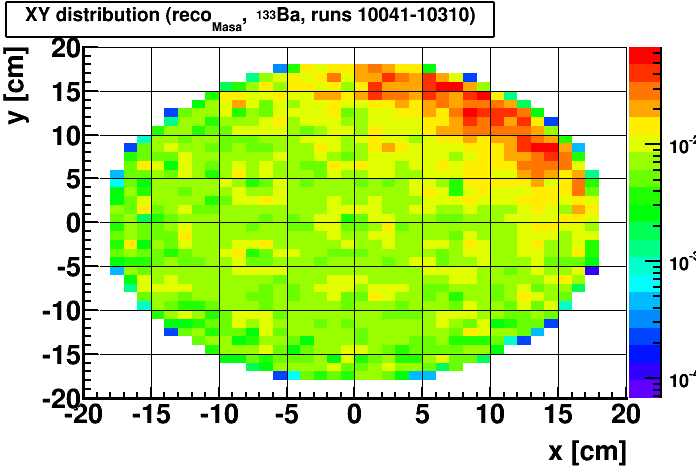
\includegraphics[width=0.43\textwidth]{./Figures/XY_Ba133_driftHV200_run10041_10310_right.png}
\caption{Two examples of XY distributions of $^{137}$Cs (left) and $^{133}$Ba (right) calibration source runs with the sources touching the cryostat from the left ($^{137}$Cs) and right ($^{133}$Ba). The $^{39}$Ar background is not subtracted and fills the TPC uniformly.
\label{fig:CalibData:XY_distrib}}
\end{figure}



\subsubsection{$^{241}$Am$^9$Be neutron data}\label{sec:CalibData:NR}

\begin{figure}[htbp]
\centering
\subfigure{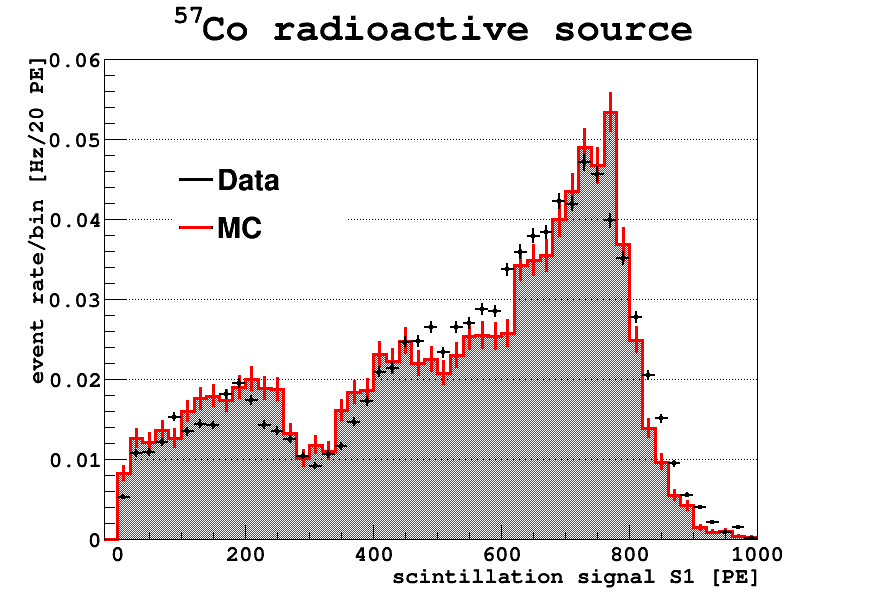
\includegraphics[width=0.51\textwidth]{./Figures/Co57_LArTPC_center.png}}
%\subfigure{\includegraphics[width=0.46\textwidth]{./Figures/F90_data_DocDB1075.png}}
\subfigure{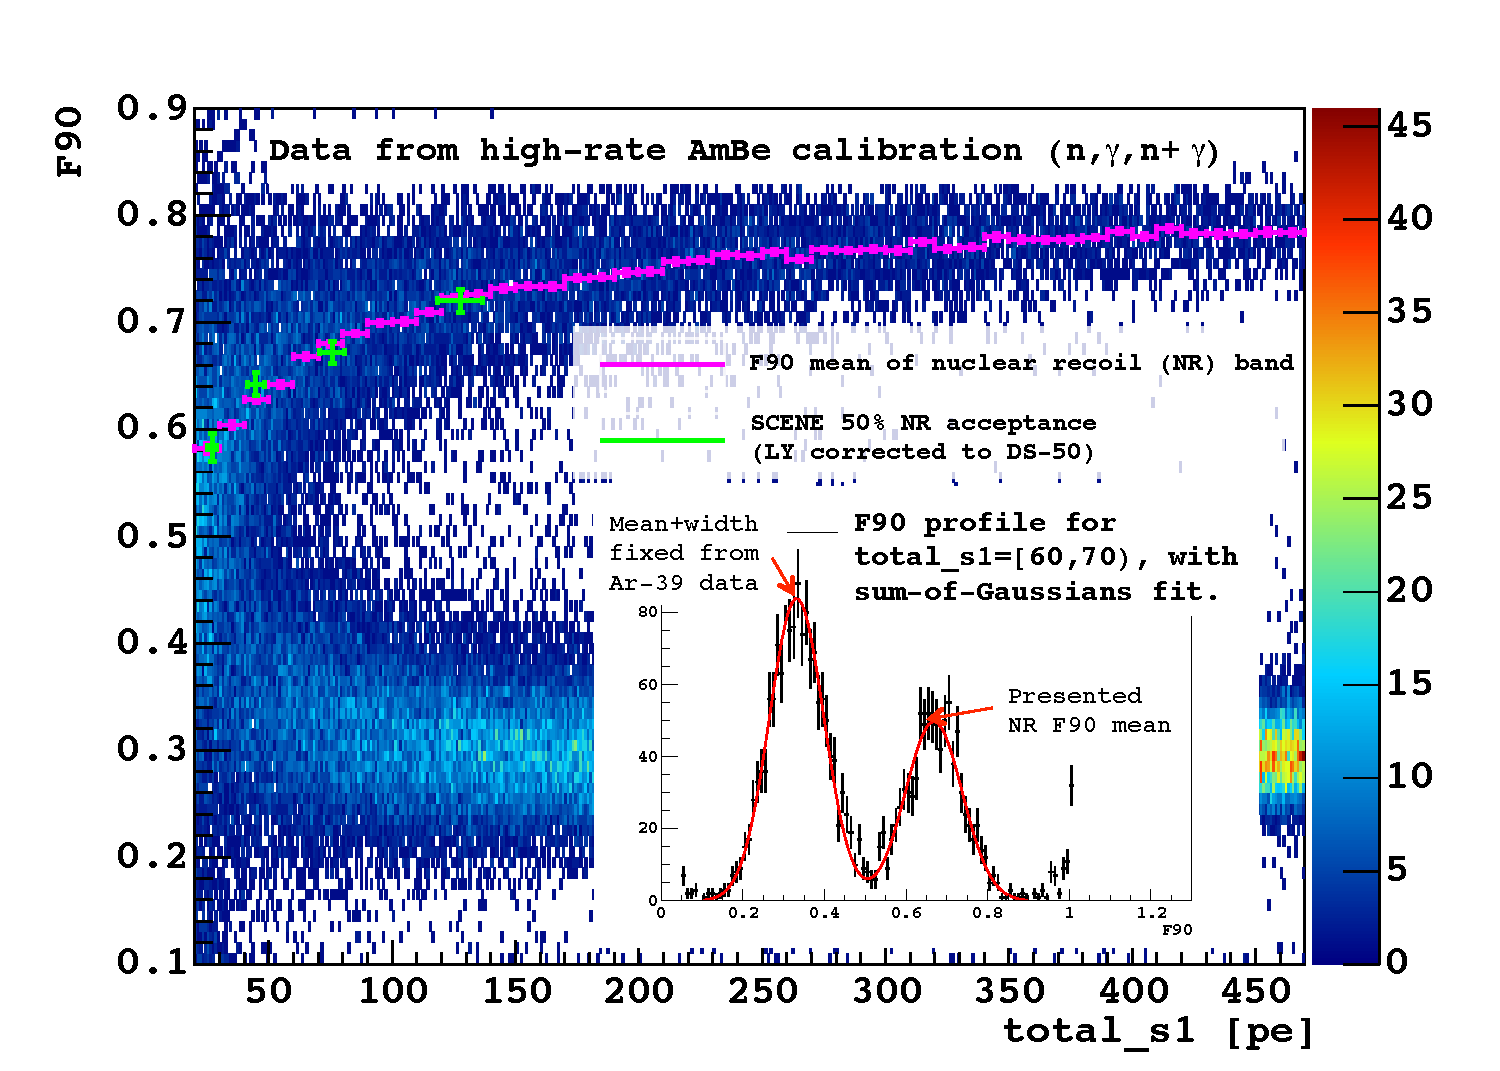
\includegraphics[width=0.47\textwidth]{./Figures/nr_f90_fit_apr2015_v8.pdf}}
 \caption{\textit{left}: Data-MC comparison for the $^{57}$Co source deployed next to the cryostat. While some improvements are yet to be made, the level of agreement between the simulation and the various complex features of the data is very encouraging.
%A lack of resolution in the MC is expected as smearing due to electronics and reconstruction effects are not taken into account in the MC. THIS DOES NOT MAKE SENSE
%\textit{right}: Distribution of pulse shape discrimination parameter F90 vs.~ S1 from \ar\ in AAr, overlayed with calibration data from $^{57}$Co and $^{133}$Ba sources. Good agreement with  the internal $^{39}$Ar illustrates the consistency of the calibration data.
\textit{right:} Plot of F90 vs. scintillation signal S1 from a high rate AmBe neutron source calibration of \dsf.  The pink line shows the mean F90 for the nuclear recoil band, while the points in green show the F90 values scaled from SCENE measurements and used in our publication Ref.~\cite{ds:ds-50-PLB}. There is very good agreement between the two.  The high source intensity and correlated neutrons and $\gamma$-ray emission by the AmBe source contribute events outside the nuclear recoil and electron recoil bands. 
\label{fig:CalibData:F90}}
 \end{figure}


%Distributions of the F90 pulse shape parameter from $^{57}$Co and $^{133}$Ba gamma sources outside the LAr-TPC are in good agreement with those from the internal calibration provided by the \ar \, decays, demonstrating the good quality of the calibration data set (Fig.~\ref{fig:CalibData:F90}, right). 

%At the time of publication of our paper Ref. \cite{ds:ds-50-PLB},  neutron calibration data was not available.  Therefore the WIMP search box for nuclear recoils was set based on measurements of F90 in the SCENE experiment \cite{scene2}. Now, a preliminary analyses of AmBe neutron source exposures shown in Fig.~\ref{fig:CalibData:F90}, lower left proves the good agreement between the extrapolated SCENE results and actual \dsf\ data.  

The WIMP search box and nuclear recoil acceptance in our paper~\cite{ds:ds-50-PLB} were established
without the availability of neutron calibration data in \dsf.  
The mean F90 from the ScENE experiment~\cite{scene2} was scaled to the light yield of DarkSide-50, and the electron and nuclear recoil acceptance curves were determined from an analytic statistical model of the F90 distributions as a function of energy. While we have full confidence in this approach, the 
data taken in the calibration campaign with the Am-Be neutron source now allow it to be directly
verified.  The mean F90 for nuclear recoils in \dsf\ is found to agree closely with the corresponding
scaled ScENE results, as shown in Fig.~\ref{fig:CalibData:F90}, right). 
%The same figure also shows Fig.~\ref{fig:CalibData:F90}, right also shows that the data with the Am-Be source will give us the mean F90 for nuclear recoils at energies beyond those measured by ScENE. 
(The higher-than-optimal intensity of this AmBe source and its 
correlated neutron and gamma ray emissions contribute events in the plot outside the nuclear recoil and electron recoil bands.)

\subsubsection{Z and XY of source position}
Tests at LNGS established the deployment system's positioning accuracy to be about $\pm$1 cm after a 7 meter journey into the DarkSide-50 detector.
%comment to the "about $\pm ": the tilde $~ \pm$ did not show up at all in the output.

 %Our first results show that the source can be positioned after its 7 meter journey into the DarkSide-50 detector with an accuracy of $~ \pm $1 cm.


This result is being validated using calibration campaign data in an ongoing analysis. 


\subsection{Liquid Scintillator Veto}\label{sec:LSV:gammasources}

In January and February 2015 the reconstitution of the LSV scintillator was completed and a second AmBe neutron source calibration of the LSV calibration was undertaken to further study the various
neutron detection channels in the LSV. With a borated scintillator, a critical aspect of the neutron detection efficiency is the capability to observe the \brbortenground\
capture branch leading to a \enbortengroundalpha\ $\alpha$ + $^7$Li(g.s.) without the accompanying 478 keV $\gamma$-ray. Veto results are described in further detail below in Sec.~\ref{sec:veto}.



\subsection{Impact of Calibration Source Deployment on Stability and Radioactivity in LY}
\section{Conclusions}\label{sec:Conclusions}\label{sec:Conclusion}
CALIS is a simple and affordable, yet effective source deployment system that has been successfully used to deploy sources in the LSV and next to the TPC and to conduct several successful calibration campaigns. No adverse effects on the LSV or TPC have been noticed.

%summarize that the LSV and TPC detector have not been negatively affected.
%that's a sentence for the summary: The critical contribution by CALIS is the neutron veto detection efficiency calibration using dedicated neutron sources
%neutron gun inside a dedicated deployment device currently under development (Section \ref{sec:Outlook}).
%Refer to the next generation DS-detector.
%\section{Epilogue}\label{sec:Epilogue}
%here I would list all upcoming DarkSide papers and how they are in relationship with each other. Since so many papers are in preparation I would find that %helpful. Even if it is not eventually put into the paper.

%%%%%%%%%%%%%%%%%%%%%%%%%%%%%%%%%%%%%
%%%%%%%%%%%%%%%%%%%%%%%%%%%%%%%%%%%%%

\section{Acknowledgements}\label{sec:Acknowledgements}
\mymarginpar{This is a verbatim copy from the veto paper - adjustments needed?}The DarkSide-50 Collaboration would like to thank LNGS laboratory and its staff for invaluable technical and logistical support. This report is based upon work supported by the US NSF (Grants PHY-0919363, PHY-1004072, PHY-1004054, PHY-1242585, PHY-1314483, PHY-1314507 and associated collaborative grants; grants PHY-1211308 and PHY-1455351), the Italian Istituto Nazionale di Fisica Nucleare (INFN), the US DOE (Contract Nos. DE-FG02-91ER40671 and DE-AC02-07CH11359), and the Polish NCN (Grant UMO-2012/05/E/ST2/02333). We thank the staff of the Fermilab Particle Physics, Scientific and Core Computing Divisions for their support. We acknowledge the financial support from the UnivEarthS Labex program of Sorbonne Paris Cit\'{e} (ANR-10-LABX-0023 and ANR-11-IDEX-0005-02) and from the S\~{a}o Paulo Research Foundation (FAPESP).
%\input{acknowledgments.tex}

%% The Appendices part is started with the command \appendix;
%% appendix sections are then done as normal sections
%% \appendix

%% \section{}
%% \label{}

%% If you have bibdatabase file and want bibtex to generate the
%% bibitems, please use
%%
%%\bibliographystyle{elsarticle-num}
\bibliographystyle{veto-description} 
%%\bibliography{veto-description}
\bibliography{CALIS}

%% else use the following coding to input the bibitems directly in the
%% TeX file.

\end{document}
\endinput
%%
%% End of file `elsarticle-template-num.tex'.
